\documentclass[12pt,a4paper]{article}
\usepackage[a4paper, total={6in, 9in}]{geometry}
\usepackage[utf8]{inputenc}
\usepackage[german]{babel}
\usepackage[T1]{fontenc}
\usepackage{amsmath}
\usepackage{amsfonts}
\usepackage{amssymb}
\usepackage{graphicx}
\usepackage{listings}
\usepackage{color}
\usepackage{float}  % for 'H' in picture placement
\usepackage{tabularx} % for automatic linebreak in tables
\usepackage[backend=biber,
style=authoryear, % Zitierstil 
natbib=true, 
hyperref=true, % hyperref-Paket für Links
maxbibnames=9, 
firstinits=true,
]{biblatex}

\addbibresource{literature.bib}


\title{Seminararbeit}
\usepackage[onehalfspacing]{setspace}
\author{Manuel Theurl}
%\usepackage{scrpage2}
\usepackage{scrpage2}

\pagestyle{scrheadings}
\clearscrheadfoot
\setlength{\parindent}{0em} 
%\setfootsepline{0.2pt}

\begin{document}


%\ifoot{{\small Manuel Theurl}}
%\cfoot{{\small \today}}
%\ofoot{{\small \pagemark}}

%Titelseite:
\begin{titlepage}

\begin{flushright}
\begin{normalsize}
Seminar zur Integrativen Geographie (Ansätze in der Hydrologie), 402.212
\\
Sommersemester 2018/19
\end{normalsize}
\end{flushright}

\vspace{5cm}

\begin{center}

\includegraphics[width=0.3\textwidth]{logo_uni_graz.jpg}

\vspace{1.5cm}

\textbf{\Large Energiebilanz im Ablationsgebiet der Pasterze}\\
\vspace{2cm}
\textsc{\large {Bachelorarbeit}}\\[4cm]
\end{center}

\vspace{2cm}

\begin{flushright}
Manuel Theurl, 01610570\\
\today
\end{flushright}

\end{titlepage} 

\pagebreak
\section*{Abstract}

\pagebreak
\section*{Vorwort}

\pagebreak
\section*{Danksagung}

\pagebreak
%Inhaltsverzeichnis:
\ofoot{{\small \pagemark}}
\pagenumbering{Roman} 
\tableofcontents
\vspace{1cm}

\pagebreak
\listoffigures
\vspace{1cm}

\pagebreak
\listoftables
\vspace{1cm}


\pagebreak
\pagenumbering{arabic}  
\setcounter{page}{1}

\section{Einleitung}
Die Pasterze am Fuße des Großglockners in Österreich ist Gegenstand vieler wissenschaftlicher Untersuchungen. Durch eine Betrachtung der Energiebilanz im Ablationsgebiet dieser, soll es ermöglicht werden, das Wissen über die Pasterze und vor allem auch über das Abschmelzen dieser zu vertiefen. Durch Wetterdaten von der Wetterstation bei der Pasterze und geeignete Energiebilanz-Kalkulationen soll somit ein Modell generiert werden, dass die Vergangenheit beschreibt, die Gegenwart bestätigt und Prognosen für die Zukunft erstellt.


\section{Theoretisches Grundwissen}
Um die vorgestellte Forschungsfrage und die damit zusammenhängenden Methoden einwandfrei verstehen zu können, braucht es ein gewisses Grundwissen über die Pasterze an sich, über die Energiebilanz sowie über das Phänomen ``Global dimming'' bzw. ``Global brigthening''.

\subsection{Pasterze und Ablationsgebiet}
Die Pasterze beim Großglockner ($3798~m$) ist trotz der Abschmelztendenzen nach wie vor der größte Gletscher der Ostalpen. Messungen aus dem Jahre 2006 ergeben eine damalige Länge von $8.3~km$, eine Fläche von $17.3~km^2$ und ein Volumen von $1.7~km^3$ (vgl. \cite[10]{Pasterze}). Der Großglockner und die Pasterze stellen eine ``fachlich perfekte'' Modellregion dar und sind damit wohl stark für die ``österreichische Bergästhetik'' verantwortlich (vgl. \cite[13]{Pasterze}).\\
Die Pasterze hatte um das Jahr 1850 ihren Höchststand. Seit diesem Zeitpunkt nimmt die Eismasse sowie die Gletscherlänge, wie in Abbildung \ref{fig:Längenverluste der Pasterze} ersichtlich, aufgrund klimatischer Veränderungen stetig ab (vgl. \cite[17]{Pasterze}).\\

Die kleine Eiszeit von ca. 1260-1860 zerstörte (durch den Hochstand 1850) Spuren von früheren Vorstößen wie zum Beispiel Moränen. Funde von Holz und Torf vor dem aktuellen Eisrand ergaben jedoch ein Alter von 9000 Jahren, was bedeutet, dass die Pasterze schon zumindest seit dem frühen Holozän existiert (vgl. \cite[24]{Pasterze}).

Folgende Abbildung zeigt einen Überblick vom Großglockner, den umliegenden Bergen und der Pasterze. 
\begin{figure}[H]
\centering
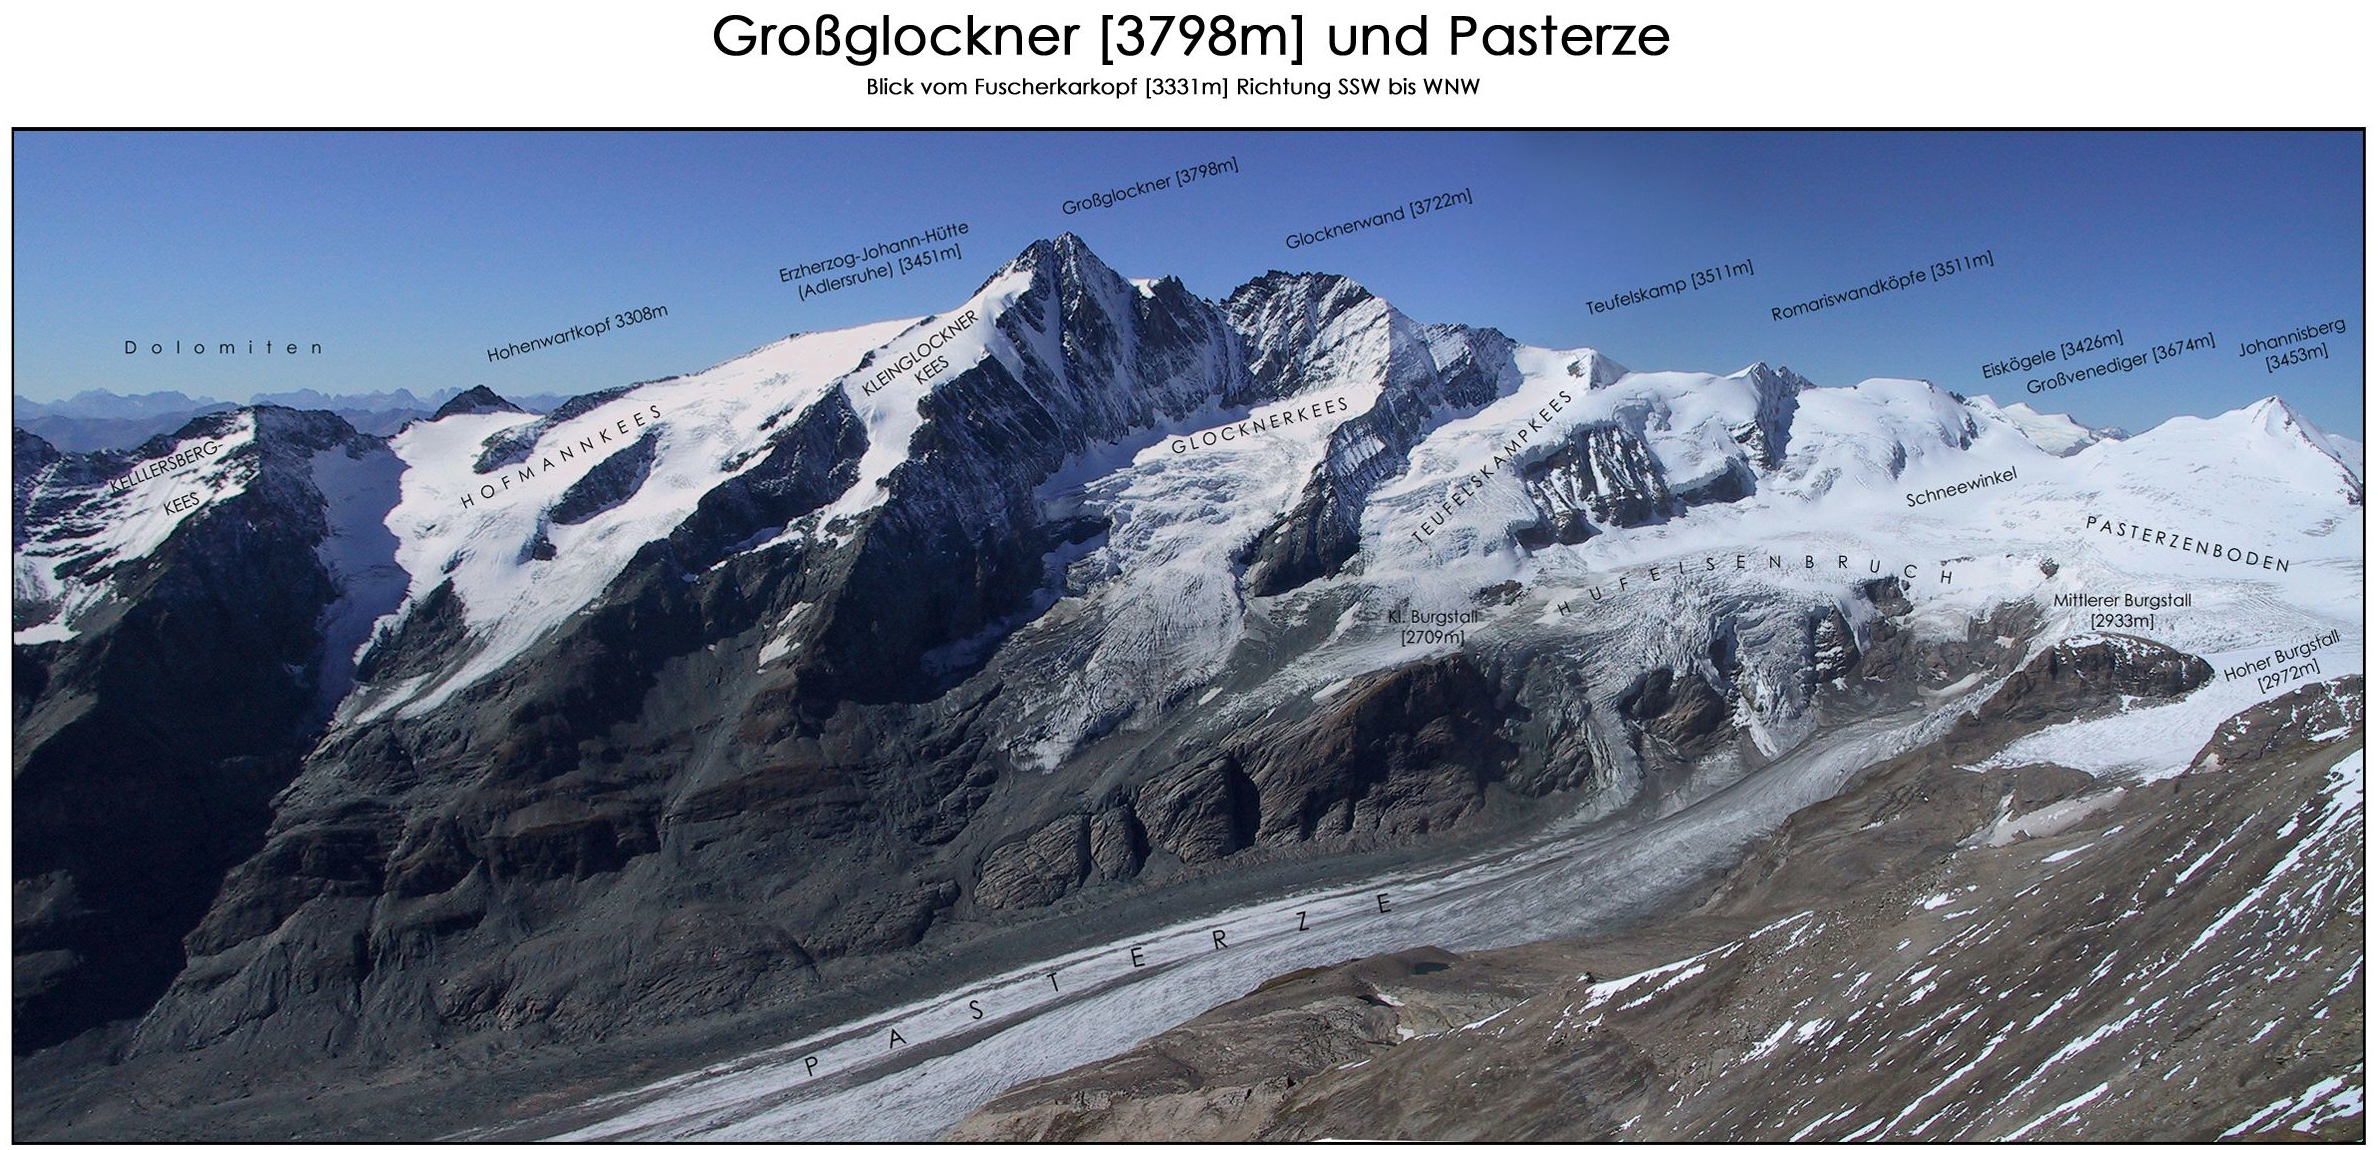
\includegraphics[width=1\textwidth]{pictures/Pasterze_Beschriftung_bw.jpg}
\caption[Großglockner und Pasterze]{Großglockner und Pasterze (Fotos: Gerhard K. Lieb vom 22.09.2006, Bildbearbeitung: Ulf Oberth)}
\label{fig:Grossglockner und Pasterze}
\end{figure}
\pagebreak
Der erwähnte Längenverlust wird mit folgender Abbildung ersichtlich.

% cited correctly??
\begin{figure}[H]
\centering
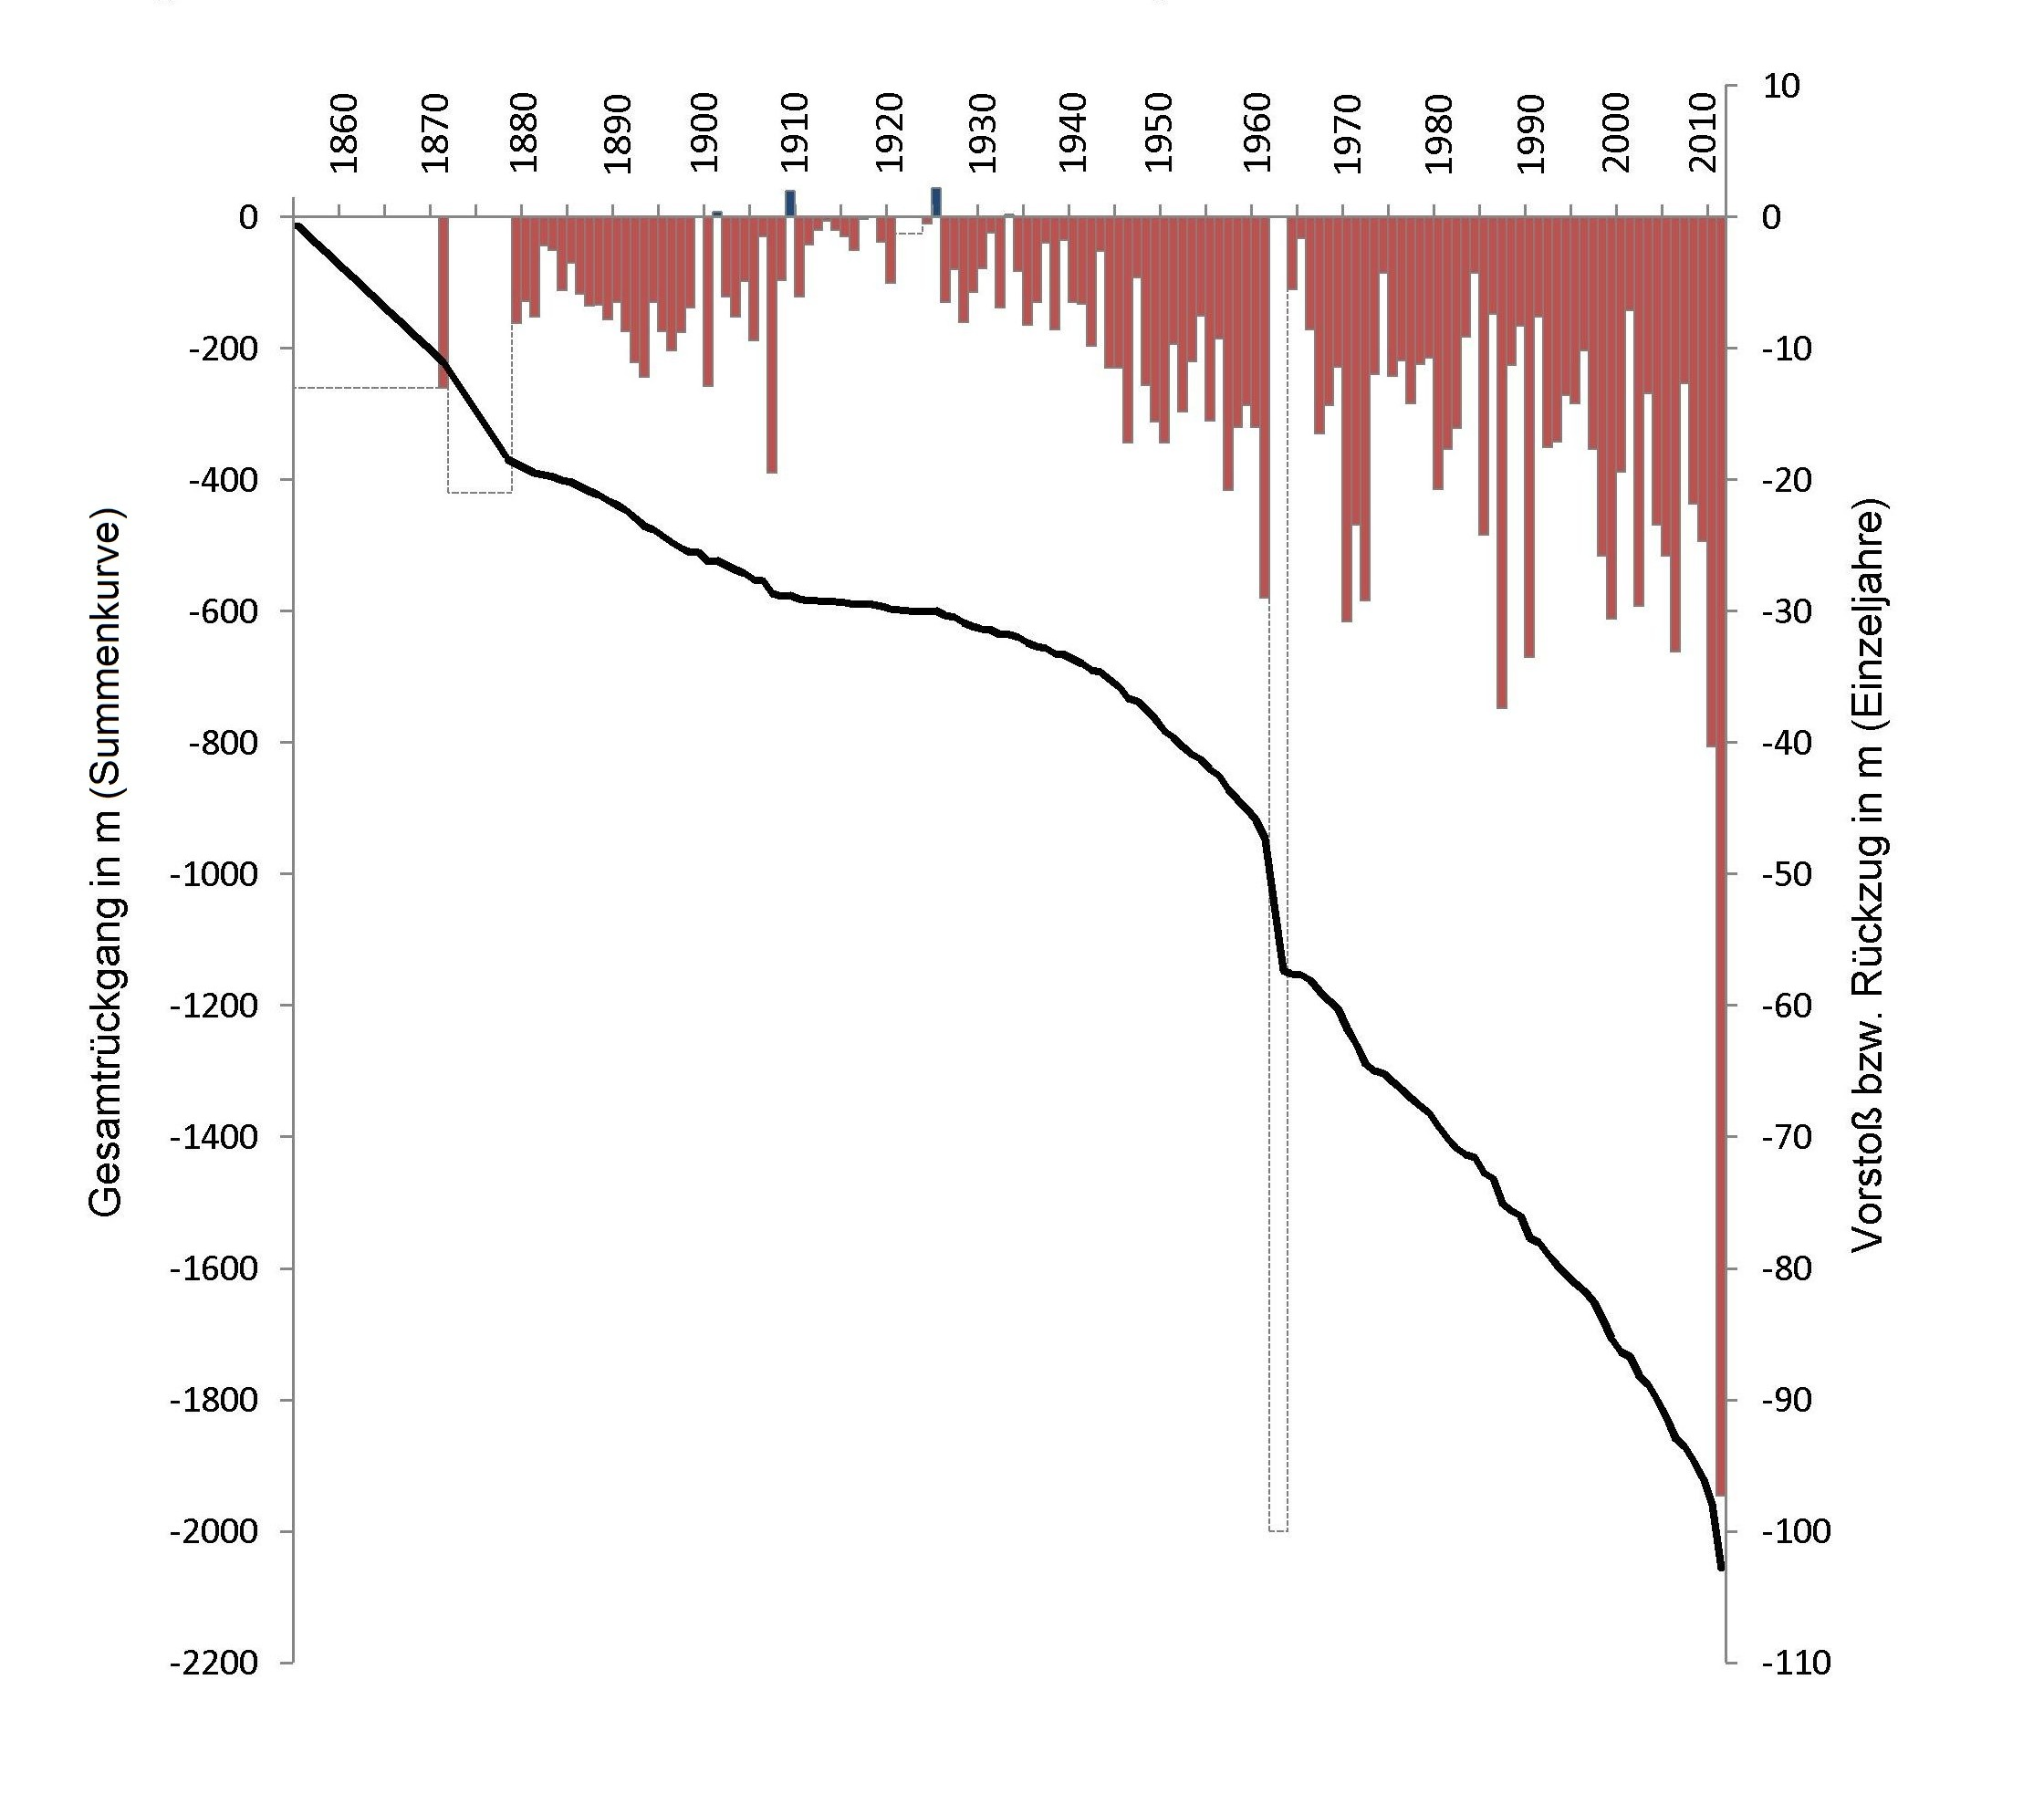
\includegraphics[width=1\textwidth]{pictures/pasterze_laengenaenderung.jpg}
\caption[Längenverluste der Pasterze nach Einzeljahren und in Summe seit 1856]{Längenverluste der Pasterze nach Einzeljahren und in Summe seit 1856  (Quelle:  \cite{LaengenaenderungPasterze})}
\label{fig:Längenverluste der Pasterze}
\end{figure}


\subsection{Energiebilanz}
\subsubsection{Energiebilanz Komponenten}\label{Energiebilanz Komponenten}
Um die Energiebilanz in der oberen Schicht eines Gletschers zu verstehen, müssen die einzelnen Komponenten, welche einen Einfluss auf die Energiebilanz haben, betrachtet werden. Abbildung \ref{fig:Energiebilanz Komponenten} gibt einen Überblick über diese Komponenten.

\begin{figure}[H]
\centering
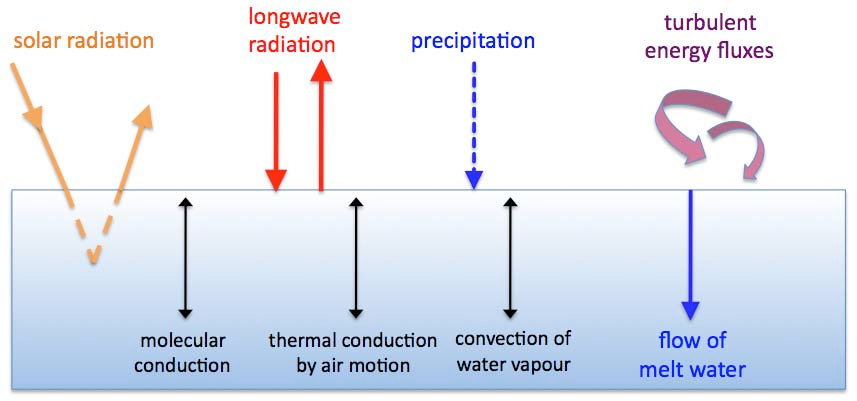
\includegraphics[width=1\textwidth]{pictures/energy_balance_components.png}
\caption[Energiebilanz Komponenten]{Energiebilanz Komponenten \parencite{Themicroclimateofvalleyglaciers}}
\label{fig:Energiebilanz Komponenten}
\end{figure}

Den größten Anteil am Energiefluss hat die kurzwellige Sonnenstrahlung. Typischerweise liegt dieser Anteil bei ein paar Hundert Watt pro Quadratmeter. Je nach Beschaffenheit der Gletscheroberfläche wird mehr oder weniger dieser kurzwelligen Strahlung reflektiert. Der Prozentsatz, welcher angibt, wie viel Strahlung reflektiert wird, wird mit Albedo bezeichnet (siehe Kapitel \ref{Albedo}). Jener Teil, der nicht reflektiert wird, dringt in den Gletscher ein, wirkt sich also positiv auf die Energiebilanz aus.\\

Langwellige Strahlung wird (fast) vollständig vom Gletscher absorbiert. Der Gletscher strahlt gleichzeitig aber auch langwellige Strahlung wieder ab. Bei warmen Temperaturen, hoher Luftfeuchtigkeit und Präsenz von Wolken, ist die Bilanz der langwelligen Strahlung positiv, ansonsten ist sie im Normalfall negativ.\\
Wolken führen nämlich dazu, dass weniger kurzwellige Sonnenstrahlung und mehr langwellige Strahlung zur Gletscheroberfläche gelangt. Für die Energiebilanz ist dabei aber noch wichtig zu wissen, ob der Gletscher ein hohes Albedo (z.B. Neuschnee) oder niedriges Albedo (z.B. Eis) aufweist. Ein hohes Albedo würde dazu führen, dass der Großteil an kurzwelliger Strahlung reflektiert wird. Nimmt also die Bewölkung zu, so gibt es mehr langwellige Strahlung die trotzdem absorbiert werden kann. Daraus folgt eine positive Auswirkung auf die Energiebilanz.\\
Simultan dazu wirkt sich Bewölkung bei niedrigem Albedo negativ auf die Energiebilanz aus. Der kurzwellige Strahlungseffekt würde dabei nämlich dem langwelligen überwiegen, da kurzwellige Strahlung energiereicher ist als langwellige.\\

Ob sich der Niederschlag positiv oder negativ auf die Energiebilanz des Gletschers auswirkt hängt von der Temperatur von diesem ab. Je nachdem ob die Temperatur höher oder niedriger ist als die Gletscheroberflächentemperatur ist die Auswirkung positiv oder negativ. Die Energieflüsse, welche hier wirken, sind aber sehr klein.\\

Turbulente Energieflüsse zwischen der Gletscheroberläche und der Atmosphäre wirken sich signifikant auf den Energiefluss aus. Grundvoraussetzung für diese turbulenten Energieflüsse ist, dass die Lufttemperatur über dem Gefrierpunkt liegt. Grund dafür ist, dass die Energieflussrichtung im Gletscher dem Gradienten der Temperatur entspricht, was bedeutet, dass der Energiefluss in Richtung der Gletscheroberfläche verläuft. Je nach dem wie hoch die Lufttemperatur und wie hoch die Luftfeuchtigkeit ist, kann nun entweder durch Verdunstung Kälte oder durch Kondensation Wärme entstehen. Bei einer Lufttemperatur von $10^\circ C$ beispielsweise, stellt die relative Feuchtigkeit von $50~\%$ den Wendepunkt zwischen positiver ($>50~\%$) und negativer ($<50~\%$) Auswirkung auf die Energiebilanz dar.\\

Der Fluss von Schmelzwasser innerhalb des Gletschers stellt einen latenten Wärmefluss dar. 
``Molecular conduction'' bezeichnet die Wärmeleitung durch Kollision von mikroskopisch kleinen Partikeln. Die Reibungshitze wirkt sich durch das Reiben des Eises an der Oberfläche ebenfalls positiv auf die Energiebilanz auf.\\
Kleine Energieflüsse entstehen auch noch durch Hitze- und Wasserdampftransport durch Konvektion im Schnee oder Firn. Diese Flüsse wirken sich aber vor allem auf die Metamorphose der Schneekristalle aus und sind abhängig von der Dichte des Schnees und vom Temperaturgradienten im Schnee (vgl. \cite[16, 17]{Themicroclimateofvalleyglaciers}).


\subsubsection{Albedo}\label{Albedo}
Die Albedo bezeichnet das Verhältnis zwischen rückgestrahltem und einfallendem Licht. Sie gibt also den Prozentsatz an Strahlung an, der beispielsweise vom Gletscher reflektiert wird. Folgende Abbildung gibt einen Überblick über das Rückstrahlvermögen von verschiedenen Oberflächenbedeckungen eines Gletschers.

\begin{figure}[H]
\centering
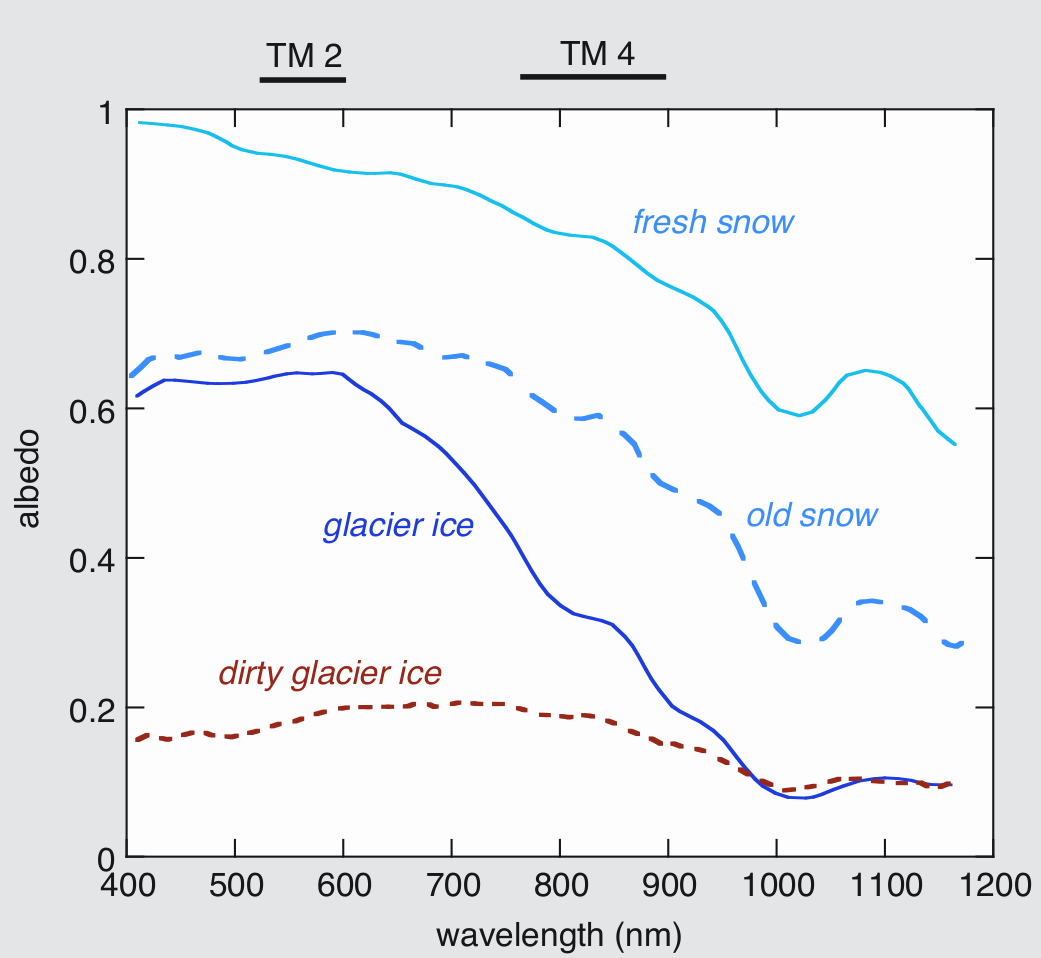
\includegraphics[width=0.8\textwidth]{pictures/spectral_reflectance_curves_for_ice_and_snow.png}
\caption[Spektrale Relektorkurven von Eis und Schnee]{Spektrale Relektorkurven von Eis und Schnee \parencite{Themicroclimateofvalleyglaciers}}
\label{fig:Spektrale Relektorkurven von Eis und Schnee}
\end{figure}

Auf der Pasterze verringert sich die Nettostrahlung welche sich positiv auf die Energiebilanz des Gletschers auswirkt mit zunehmender Höhe. Grund dafür ist eben genau die Albedo, denn Schnee bedeckt die höher liegenden Teile des Gletschers und reflektiert mehr Strahlung. Das Eis im Ablationsgebiet absorbiert sehr viel Strahlungsenergie (vgl. \cite[171]{ThePhysicsOfGlaciers}).

\subsection{``Global dimming''}
% TODO komplett weg?
Mehrere Langzeitstudien von Oberflächenstrahlungsmessungen haben gezeigt, dass die Strahlung, welche auf der Erdoberfläche ankommt im Hinblick auf eine dekadische Zeit nicht konstant ist, d.h. sich innerhalb von 10er-Jahren signifikant ändern kann. Diese Änderungen wurden unter den Begriffen ``Global dimming'' und ``Global brightening'' zusammengefasst, wobei der Begriff ``global'' sich auf die Summe von diffuser und direkter Sonnenstrahlung bezieht und nicht auf global, im Sinne von ``auf der ganzen Welt''.\\
Änderung der Oberflächenstrahlung können nicht nur bei wolkigen Bedingungen festgestellt werden, sondern auch bei einer wolkenfreien Atmosphäre. Das deutet darauf hin, dass sich der Mensch durch Einbringung von Aerosolen in die Atmosphäre auf diese Oberflächenstrahlung auswirkt (vgl. \cite[1]{GlobalDimming}).\\
Aerosole können diese Oberflächenstrahlung verändern, indem sie die Sonnenstrahlen streuen oder absorbieren. Weiters können die Aerosole als Kondensationskerne bei der Wolkenbildung agieren und somit diese fördern. Insgesamt reduzieren also Aerosole die Oberflächenstrahlung. Eine der Hauptursachen von ``global dimming'' ist somit die Erzeugung von Aerosolen durch die Industrie (vgl. \cite[14]{GlobalDimming}).\\ 
Die Oberflächenstrahlung bzw. die kurzwellige Sonnenstrahlung spielt, wie bereits in Kapitel \ref{Energiebilanz Komponenten} erwähnt, eine große Rolle in der Energiebilanz der Gletscher. Auf der Nordhalbkugel sei zu beobachten gewesen, dass bis zu den 1980-Jahren keine signifikanten Änderungen in den Flächenbedeckungen der Gletscher stattgefunden hat, aber ab ca. 1980 mit dem Effekt des ``global brigthening'' die Gletscher schlagartig an Größe verloren hätten (vgl. \cite[24]{GlobalDimming}).


\pagebreak
\section{Methodik}
\subsection{Berechnung der Energiebilanz}
\citeauthor{ThePhysicsOfGlaciers} (\citeyear{ThePhysicsOfGlaciers}) geben in Kapitel 5 ``Mass Balance Processes: 2. Surface Ablation and Energy Budget'' detaillierte Formeln zur Berechnung der Energiebilanz an. Ausgegangen wird von Formel 

\begin{equation}
E_{N}=\underbrace{E_{S}^{\downarrow}+E_{S}^{\uparrow}+E_{L}^{\downarrow}+E_{L}^{\uparrow}}_{E_{\mathrm{R}}}+E_{G}+E_{H}+E_{E}+E_{P},
\end{equation}

wobei $E_{N}$ dem Nettoenergiefluss in die Oberfläche, $E_{S}^{\downarrow}$ der ankommenden kurzwelligen Strahlung, $E_{S}^{\uparrow}$ der reflektierten kurzwelligen Strahlung, $E_{L}^{\downarrow}$ der ankommenden langwelligen Strahlung, $E_{L}^{\uparrow}$ der reflektierten langwelligen Strahlung $E_{G}$ dem Energiefluss unter der Oberfläche, $E_{P}$ dem Energieeintrag durch Niederschlag und $E_{H}$ und $E_{E}$ den spürbaren und latenten Wärmeflüssen durch Zirkulation entsprechen. $E_{\mathrm{R}}$ ist die Summe aller Strahlungen und gibt somit die Nettostrahlung an (positiv für Energieeintrag in den Gletscher).\\

Ausgehend von dieser Grundgleichung beschreibt \citeauthor{ThePhysicsOfGlaciers} weitere Aspekte die zu berücksichtigen sind, wie zum Beispiel 

\begin{itemize}
\item{Schmelzrate, abhängig auch von Dicke }
\item{Wiedergefrieren von Schmelzwasser in den unteren Schichten erzeugt Wärme}
\item{Abhängigkeit der kurzwelligen Strahlung vom Einfallwinkel und von der atmosphärischen Durchlassungsfähigkeit}
\end{itemize}

Um die spürbaren und latenten Wärmeflüsse $E_{H}$ und $E_{E}$ zu berechnen, schildern \citeauthor{ThePhysicsOfGlaciers} eine Berechnungsmethode über den ``Bulk Aerodynamic Approach'' und die ``Flux-gradient Theory'' (vgl. \cite[153-157]{ThePhysicsOfGlaciers}).\\
Die genaue Herleitung dieser Formeln kann dort nachgelesen werden, als Ergebnis folgen schlussendlich aber die zwei Formeln

\begin{equation}\label{Berechnung latenter Energiefluss}
E_{E}= 22.2~C^*~\mu(z)~(e_a-e_s)
\end{equation}

für den latenten und

\begin{equation}\label{Berechnung sensibler Energiefluss}
E_{H}= 0.0129~C^*~P~\mu(z)~(T_a(z)-T_s)
\end{equation}

für den sensiblen Wärmefluss. $C^*$ ist dabei der Transferkoeffizient und wird mit 

\begin{equation}
C^{*}=\frac{k_{o}^{2}}{\ln ^{2}\left(z / z_{0}\right)}
\end{equation}

% TODO Pfad
berechnet, wobei $k_{o}=0.4$ die Karmans Konstante, $z_{0}$ die Messhöhe über dem Eis ist, in welcher die Windgeschwindigkeit gemessen wird und $z=0.003~m$ dem Rauheitsparameter entspricht. Tabelle 5.4 in Cuffey und Paterson 2010 zeigt, dass dieser Parameter bei Eis im Ablationsgebiet zwischen 1 und 5 Millimetern beträgt. Deshalb wird er in den Berechnungen hier mit dem Mittelwert 3 Millimeter angenommen.\\ % evtl footnote bei Karmans Konstante TODO?

$T_s$ entspricht der Oberflächentemperatur des Eises und wird mithilfe vom Stefan-Boltzmann-Gesetz 

\begin{equation}
I = e \cdot \sigma \cdot T^4
\end{equation}

berechnet. $e$ entspricht der Emissivität, welche laut TODO bei Eis im Infrarotbereicht ca. 1 ist. $\sigma=5.670 \cdot 10^{-8}$ entspricht der Stefan-Boltzmann-Konstante und $T$ der Oberflächentemperatur des Körpers. $I$ ist die abgestrahlte Energie in $W/m^2$ welche hier in Form der langwelligen Ausstrahlung gegeben ist. Somit folgt durch Umstellungen die Oberflächentemperatur

\begin{equation}\label{eq:Oberflächentemperatur}
T = \sqrt[4]{\frac{I}{\sigma}}
\end{equation}


$e_a$ entspricht dem tatsächlichen Wasserdampfdruck in der Luft und wird aus dem Sättigungswasserdampfdruck


\begin{equation}
e_{a_{saturated}}=0.6108 \cdot e^{17.27 \cdot \frac{T_a}{T_a + 237.3}}
\end{equation}

durch

\begin{equation}
e_a = \frac{rel_{humidty}}{100} \cdot e_{a_{saturated}}
\end{equation}

berechnet. $T_a$ entspricht dabei der Lufttemperatur in Grad Celsius und die Einheit des Ergebnisses $e_a$ ist $kPa$.\\

$e_s$ wird analog zu $e_a$ berechnet, nur dass statt der Lufttemperatur $T_a$ die mit Formel \ref{eq:Oberflächentemperatur} berechnete Eisoberflächentemperatur verwendet wird.\\
$\mu(z)$ und $T_a(z)$ stehen für die Windgeschwindigkeit und Lufttemperatur gemessen in Höhe $z$, $P$ für den Luftdruck in Einheit Pascal.


\subsection{Periodische Trendelimination}
Im Falle der Pasterze liegen leider nur für 3 Jahre Messdaten für die Berechnung der Energiebilanz zur Verfügung. Deshalb kann durch eine periodische Trendelimination keine aussagekräftige Annahme über eventuellen Trend getroffen werden. Trotzdem wird die Möglichkeit zur periodischen Trendelimination in die Software implementiert, um z.B. bei anderen Gletschern und längeren Datenaufzeichnungen bzw. in Zukunft auch bei der Pasterze Trendanalysen durchzuführen.\\

Eine Periode dauert bei der Energiebilanz genau ein Jahr. Die Bereinigung von der Periode erfolgt auf die Weise, dass der erste Wert nach dem vollendeten Jahr vom Wert im ersten Jahr zu dieser Zeit abgezogen wird. Es wird dabei immer jener Wert vom ersten Jahr gesucht, welcher datumsmäßig (abzüglich von der Jahresanzahl) am nächsten zum betrachteten Wert liegt. Dieser Vorgang wird für alle weiteren Werte wiederholt. Soll ein eventueller linearer Trend erhalten bleiben, so müssen die Werte immer bezogen auf das erste Jahr abgezogen werden. Wird nämlich immer nur das Vorjahr dafür verwendet, so fällt dieser lineare Trend auch noch weg. In diesem Fall könnten dann die enstandenen Residuen auf Normalverteilung überprüft werden.\\
In diesem Fall soll aber der lineare Trend eben aufrecht erhalten bleiben. Aus der genannten Methode folgt somit, dass die Werte Reihe zumindest größer als ein Jahr sein muss, ansonsten kann kein periodischer Trend eliminiert werden.\\

Im Zuge der Durchführung wird nicht nur die errechnete Energiebilanz an sich trendeliminiert, sonder auch Einzelteile, wie z.B. nur die Strahlungsenergie und nur der sensible und latente Hitzeeintrag.


\subsection{Berechnung des resultierenden Schmelzwassers}
Formel (vgl. \cite[142]{ThePhysicsOfGlaciers})


gibt einen Zusammenhang zwischen Nettoenenergiebilanz und der Schmelzrate TODO vom Gletschereis. Wenn die Temperatur im betrachteten Eislayer den Schmelzpunkt erreicht hat, dann fällt der zweite Term der Gleichung durch


blabla = 0

weg. Um die errechnete Energiebilanz auf Plausibilität zu überprüfen, indem die gemessene Ablation (später umgerechnet in Schmelzwasser) mit dem modellierten Schmelzwasser verglichen wird, reicht es für diese Analyse aus, nur den Zeitraum von 1. Juni bis 1. September zu betrachten. In diesem Zeitraum kann deshalb von einem isothermen Eislayer mit Temperatur beim Schmelzpunkt ausgegangen werden.

$f_r$ bezeichnet den Anteil vom Schmelzwasser, der im Eislayer wiedergefriert. Es folgt somit die für diese Fragestellung relevante Nettoablationsrate 

ms 1- fr TODO
Formel

, wobei TODO GRÖßEN ERKLÄREN

Die errechnete Nettoablationsrate hat die Einheit $m^3/\delta t$, mit

FORMEL * 1000

folgt somit das tatsächliche Schmelzwasser über einen gewissen Zeitraum in Liter.

Durch 

Formel

kann die gemessene Ablation ebenfalls in Schmelzwasseräquivalent umgerechnet werden.\\

Analog dazu kann auch das modellierte Schmelzwasser durch

Formel

noch in Ablation bzw. Eisdickenverlust umgerechnet werden.


\subsection{Programmierung in Python}
\subsubsection{Umgebung}

Die entwickelte Software wurde im Programm Pycharm Professional Edition objektorientiert geschrieben. Die verwendete Python Version ist Python 3.6.\\\\
Die verwendeten Module und deren Zweck in der Software werden in folgender Tabelle erklärt:


\begin{table}[H]
\centering
\setstretch{1.3} 
\caption{Python Module mit Erklärung}
\label{tab:Python Module}
\begin{tabular}{|l|l|}
\hline
\textbf{Modul} & \textbf{Zweck}                                \\ \hline
tkinter             & Erstellung des GUI         \\
os             & Ordnerverwaltung         \\
configparser             & Verwaltung der Konfigurationsdatei         \\
numpy          & Erstellung und Handhabung von Arrays          \\
matplotlib     & Grafische Darstellung der Daten               \\
math		   & Berechnungsfunktionen (Logarithmus, Wurzel, e-Funktion, ..)   \\  
datetime		   & Verwaltung von Zeit und Datum   \\
unittest		   & Erstellung einer Testumgebung   \\  \hline


\end{tabular}
\end{table}
%setstretch is removed automatically after table again
\vspace{0.3cm}

\subsubsection{Unittesting}
Das Python Modul unittest wird dazu verwendet, Funktionen des Programmes zu überprüfen. Für diese Arbeit wird es dazu verwendet, die Richtigkeit der Formeln für die Berechnung der Energiebilanz zu gewährleisten.\\

Cuffey und Paterson bieten auf Seite 157 Testwerte und das dazugehörige Ergebnis für den Transfer Koeffizienten $C^*$ von Formel \ref{eq:TODO} und für die Berechnungen der sensiblen Hitze \ref{eq:TODO} an.


\paragraph{Transfer Koeffizient}

Bei gegebener Messhöhe zwischen 1 und 2 Metern und Oberflächenrauheit von  1 - 5 Millimetern (entspricht der Oberflächenrauheit von Eis im Ablationsgebiet, Tabelle 5.4) soll ein Wert für den Transferkoeffizienten, Formel \ref{TODO} zwischen 0.002 und 0.004 herauskommen.\\

Der Test mit einer Messhöhe von 1.5 Metern und Oberflächenrauheit von 2 Millimetern wird angenommen.

\paragraph{Sensible Hitze}
Bei gegebenem Luftdruck von $800~hPa$, Windeschgeschwindigkeit von $5~m/s$, Lufttemperatur von $5^\circ C$ und Transferkoeffizienten von $0.002$ soll das Ergebnis der sensiblen Hitze, Formel \ref{TODO}, zwischen 47 und $53~W/m^2$ liegen. \\
Weiters erwähnt ist, dass von einer schmelzenden Eisoberläche ausgegangen wird und weil die Eisoberlächentemperatur nach Stefan Boltzmann (Formel \ref{TODO}) berechnet wird, wird der Funktion als langwellige Ausstrahlung ein Wert von $1000~W/m^2$ mitgegeben, womit die Eistemperatur in der Berechnung bei 0 liegt.\\

Der Test wird wiederum angenommen.

\subsubsection{Grafisches Userinterface}
Das Grafische Userinterface (GUI) setzt sich aus den Teilen 
\begin{itemize}
\item Read
\item Scope/Energy balance
\item Sum
\item Plot
\item Download
\end{itemize}
zusammen.

In \textbf{Read} kann eine Messdatei eingelesen werden. 

\begin{figure}[H]
\centering
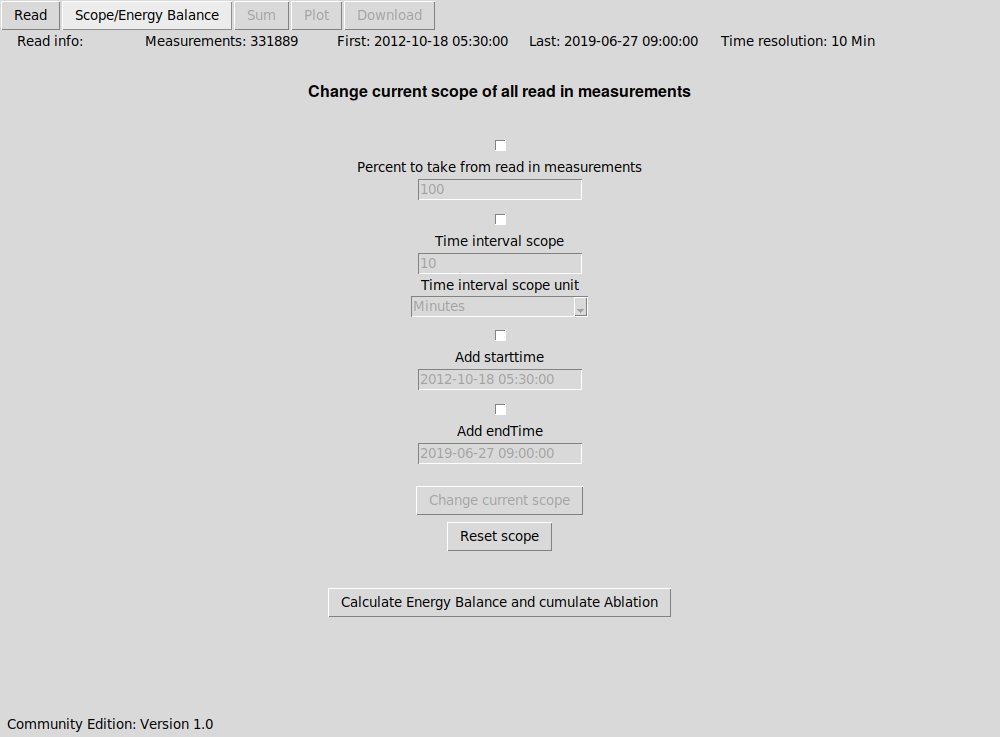
\includegraphics[width=1\textwidth]{pictures/GUI/Read_Frame.png}
\caption{GUI Read-Frame}
\label{fig:GUI Read-Frame}
\end{figure}

Im Fenster \textbf{Scope/Energy balance} kann der momentane Betrachungszeitraum verändert werden und die Energiebilanz gerechnet werden. 

\begin{figure}[H]
\centering
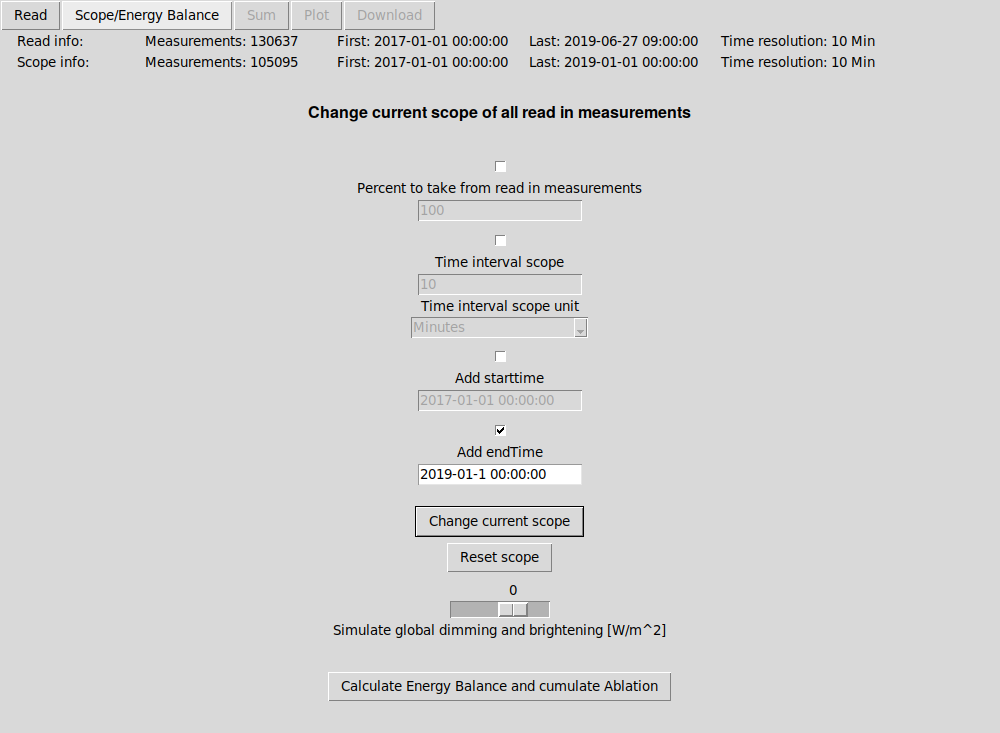
\includegraphics[width=1\textwidth]{pictures/GUI/Scope_Energy_Balance_Frame.png}
\caption{GUI Scope/Energy Balance-Frame}
\label{fig:GUI Scope/Energy Balance-Frame}
\end{figure}

Bei \textbf{Sum} können einzelne Messungen zusammengefasst werden.

\begin{figure}[H]
\centering
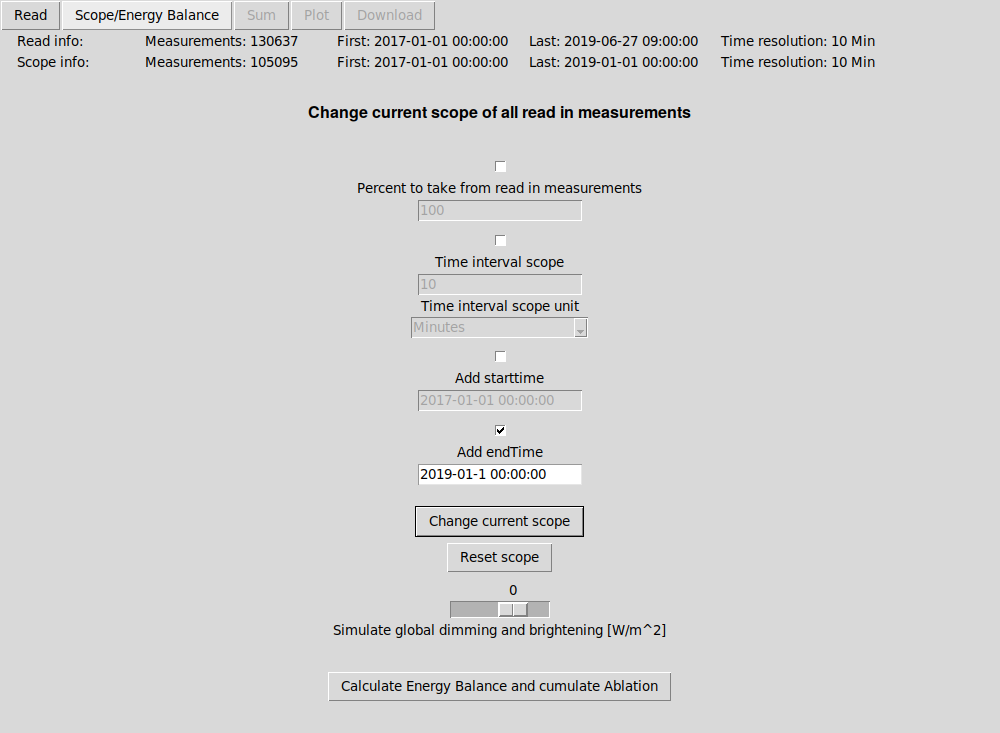
\includegraphics[width=1\textwidth]{pictures/GUI/Scope_Energy_Balance_Frame.png}
\caption{GUI Sum-Frame}
\label{fig:GUI Sum-Frame}
\end{figure}

In \textbf{Plot} können die Ergebnisse als graphische Darstellungen betrachtet werden. Es ist dabei möglich die gesamte Energiebilanz sowie deren Einzelteile zu plotten. Weiters kann die Ablation oder die errechnete gemessene und modellierte Eisschmelze als zweite Achse eingeblendet werden. Auch die Trendelimination kann visualisiert werden.

\begin{figure}[H]
\centering
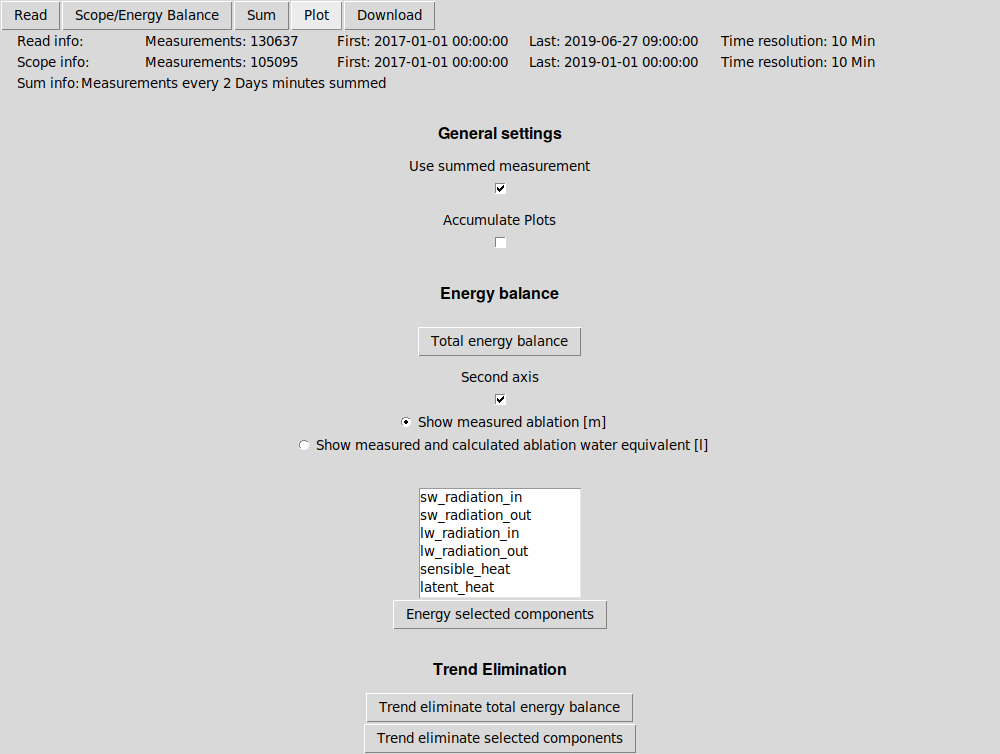
\includegraphics[width=1\textwidth]{pictures/GUI/Plot_Frame.png}
\caption{GUI Plot-Frame}
\label{fig:GUI Plot-Frame}
\end{figure}

Beim erstellen des Plots erscheint ein neues Fenster in welchem der Plots vergrößert bzw. verkleinert, verschoben, .. und heruntergeladen werden kann.

\begin{figure}[H]
\centering
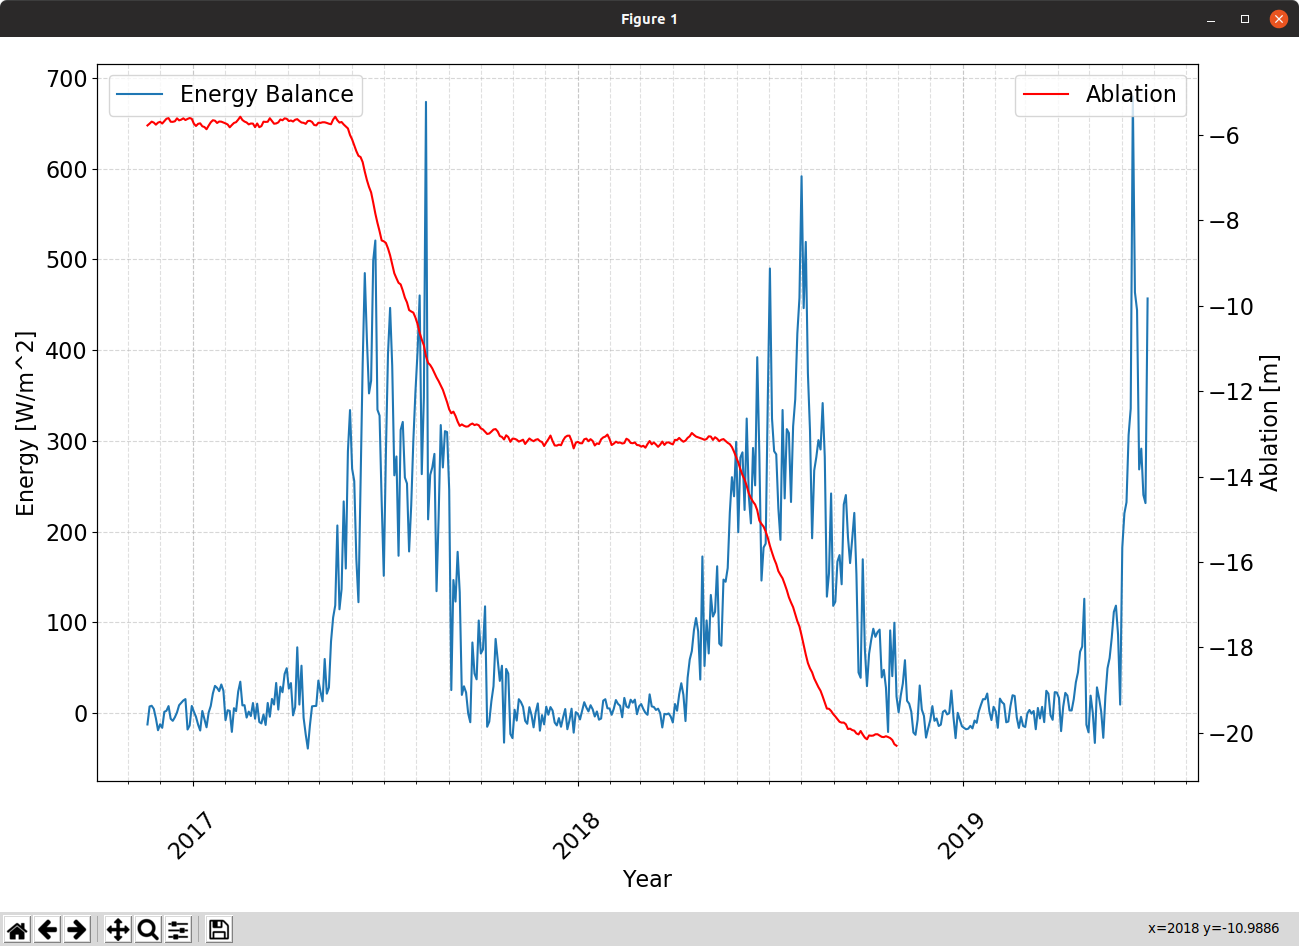
\includegraphics[width=1\textwidth]{pictures/GUI/Sample_Plot.png}
\caption{GUI Beispiel Plot}
\label{fig:GUI Beispiel Plot}
\end{figure}

Im \textbf{Download}-Bereich können die erzielten Ergebnisse noch in Form von Wertetabellen heruntergeladen werden.

\begin{figure}[H]
\centering
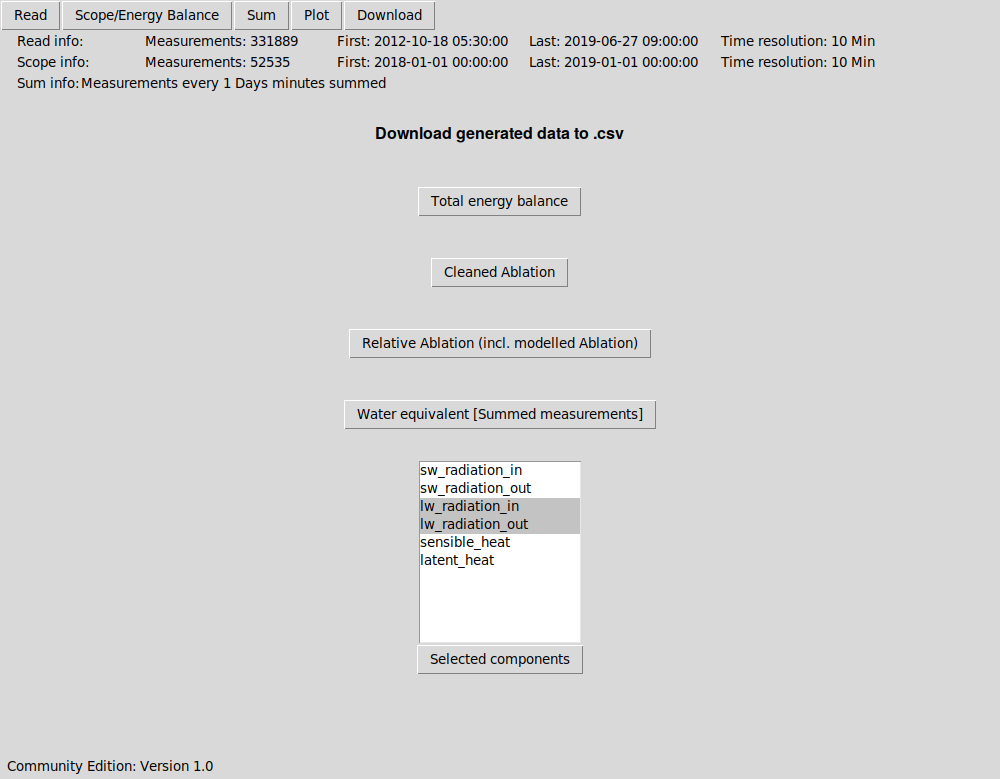
\includegraphics[width=1\textwidth]{pictures/GUI/Download_Frame.png}
\caption{GUI Download-Frame}
\label{fig:GUI Download-Frame}
\end{figure}

Eine detaillierte Beschreibung des GUI befindet sich unter TODO LINK im Wiki des Projektes auf der Platform Bitbucket.


\subsection{Softwareverwaltung}
\subsubsection{Download und Installation}
Die Open Source Version der Software ist öffentlich auf der  Platform Bitbucket unter dem Namen EnergiebilanzAblationsgebietPasterze zugänglich. Mit Klick auf Clone erscheint ein Text, der kopiert und im Terminal im gewünschten Verzeichnis ausgeführt werden muss. Git muss dafür am Rechner installiert sein.\\

Beispiel:

Terminal: \textsf{\small git clone git@bitbucket.org:atraxoo/energiebilanzablationsgebietpasterze.git}\\


Es wird nun die gesamte Software, inklusive einer Messdaten Beispieldatei heruntergeladen. Weiters wird ein Verzeichnis Exe heruntergeladen, in dem sich eine ausführbare .exe Datei befindet, womit das Programm unter Windows direkt und ohne Installation von Python ausgeführt werden kann.\\

Empfehlenswerter, vor allem im Bezug auf Updates, ist es allerdings, die Software direkt mit Python auszuführen. Dafür muss Python 3.6 oder Python 3.7 am Rechner installiert sein. Für die richtige Funktion der Software müssen gewisse Python Module installiert werden, welche sich in der requirements.txt Datei befinden. Diese Pakete können automatisiert mit dem Befehl\\

Windows Terminal: \textsf{\small pip install -r requirements.txt}\\
Linux Terminal:  \textsf{\small pip3 install -r requirements.txt}\\

installiert werden.

Optional aber empfehlenswert ist außerdem die Verwendung einer virtual environment in Python. In der offiziellen Python Dokumentation unter \textsf{\small https://docs.python.org/3/library/venv.html} ist eine Erklärung dazu zu finden.

Nachdem die Module installiert wurden, kann die Software mit \\

Windows Terminal: \textsf{\small python main.py}\\
Linux Terminal: \textsf{\small python3 main.py}\\

gestartet werden.

\subsubsection{Update}
Die aktuellste Version der Open Source Version kann mit \\

Terminal: \textsf{\small git pull} (Im Software Verzeichnis)\\

heruntergeladen werden. Zur direkt ausführbaren .exe Version gibt es keine Updates.

\pagebreak
\section{Ergebnisse und Interpretation}

Abbildung \ref{fig:Energiebilanz im gesamten Messzeitraum} zeigt die errechnete Energiebilanz über den gesamten Messzeitraum von Ende 2016 bis Mitte 2019. 

\begin{figure}[H]
\centering
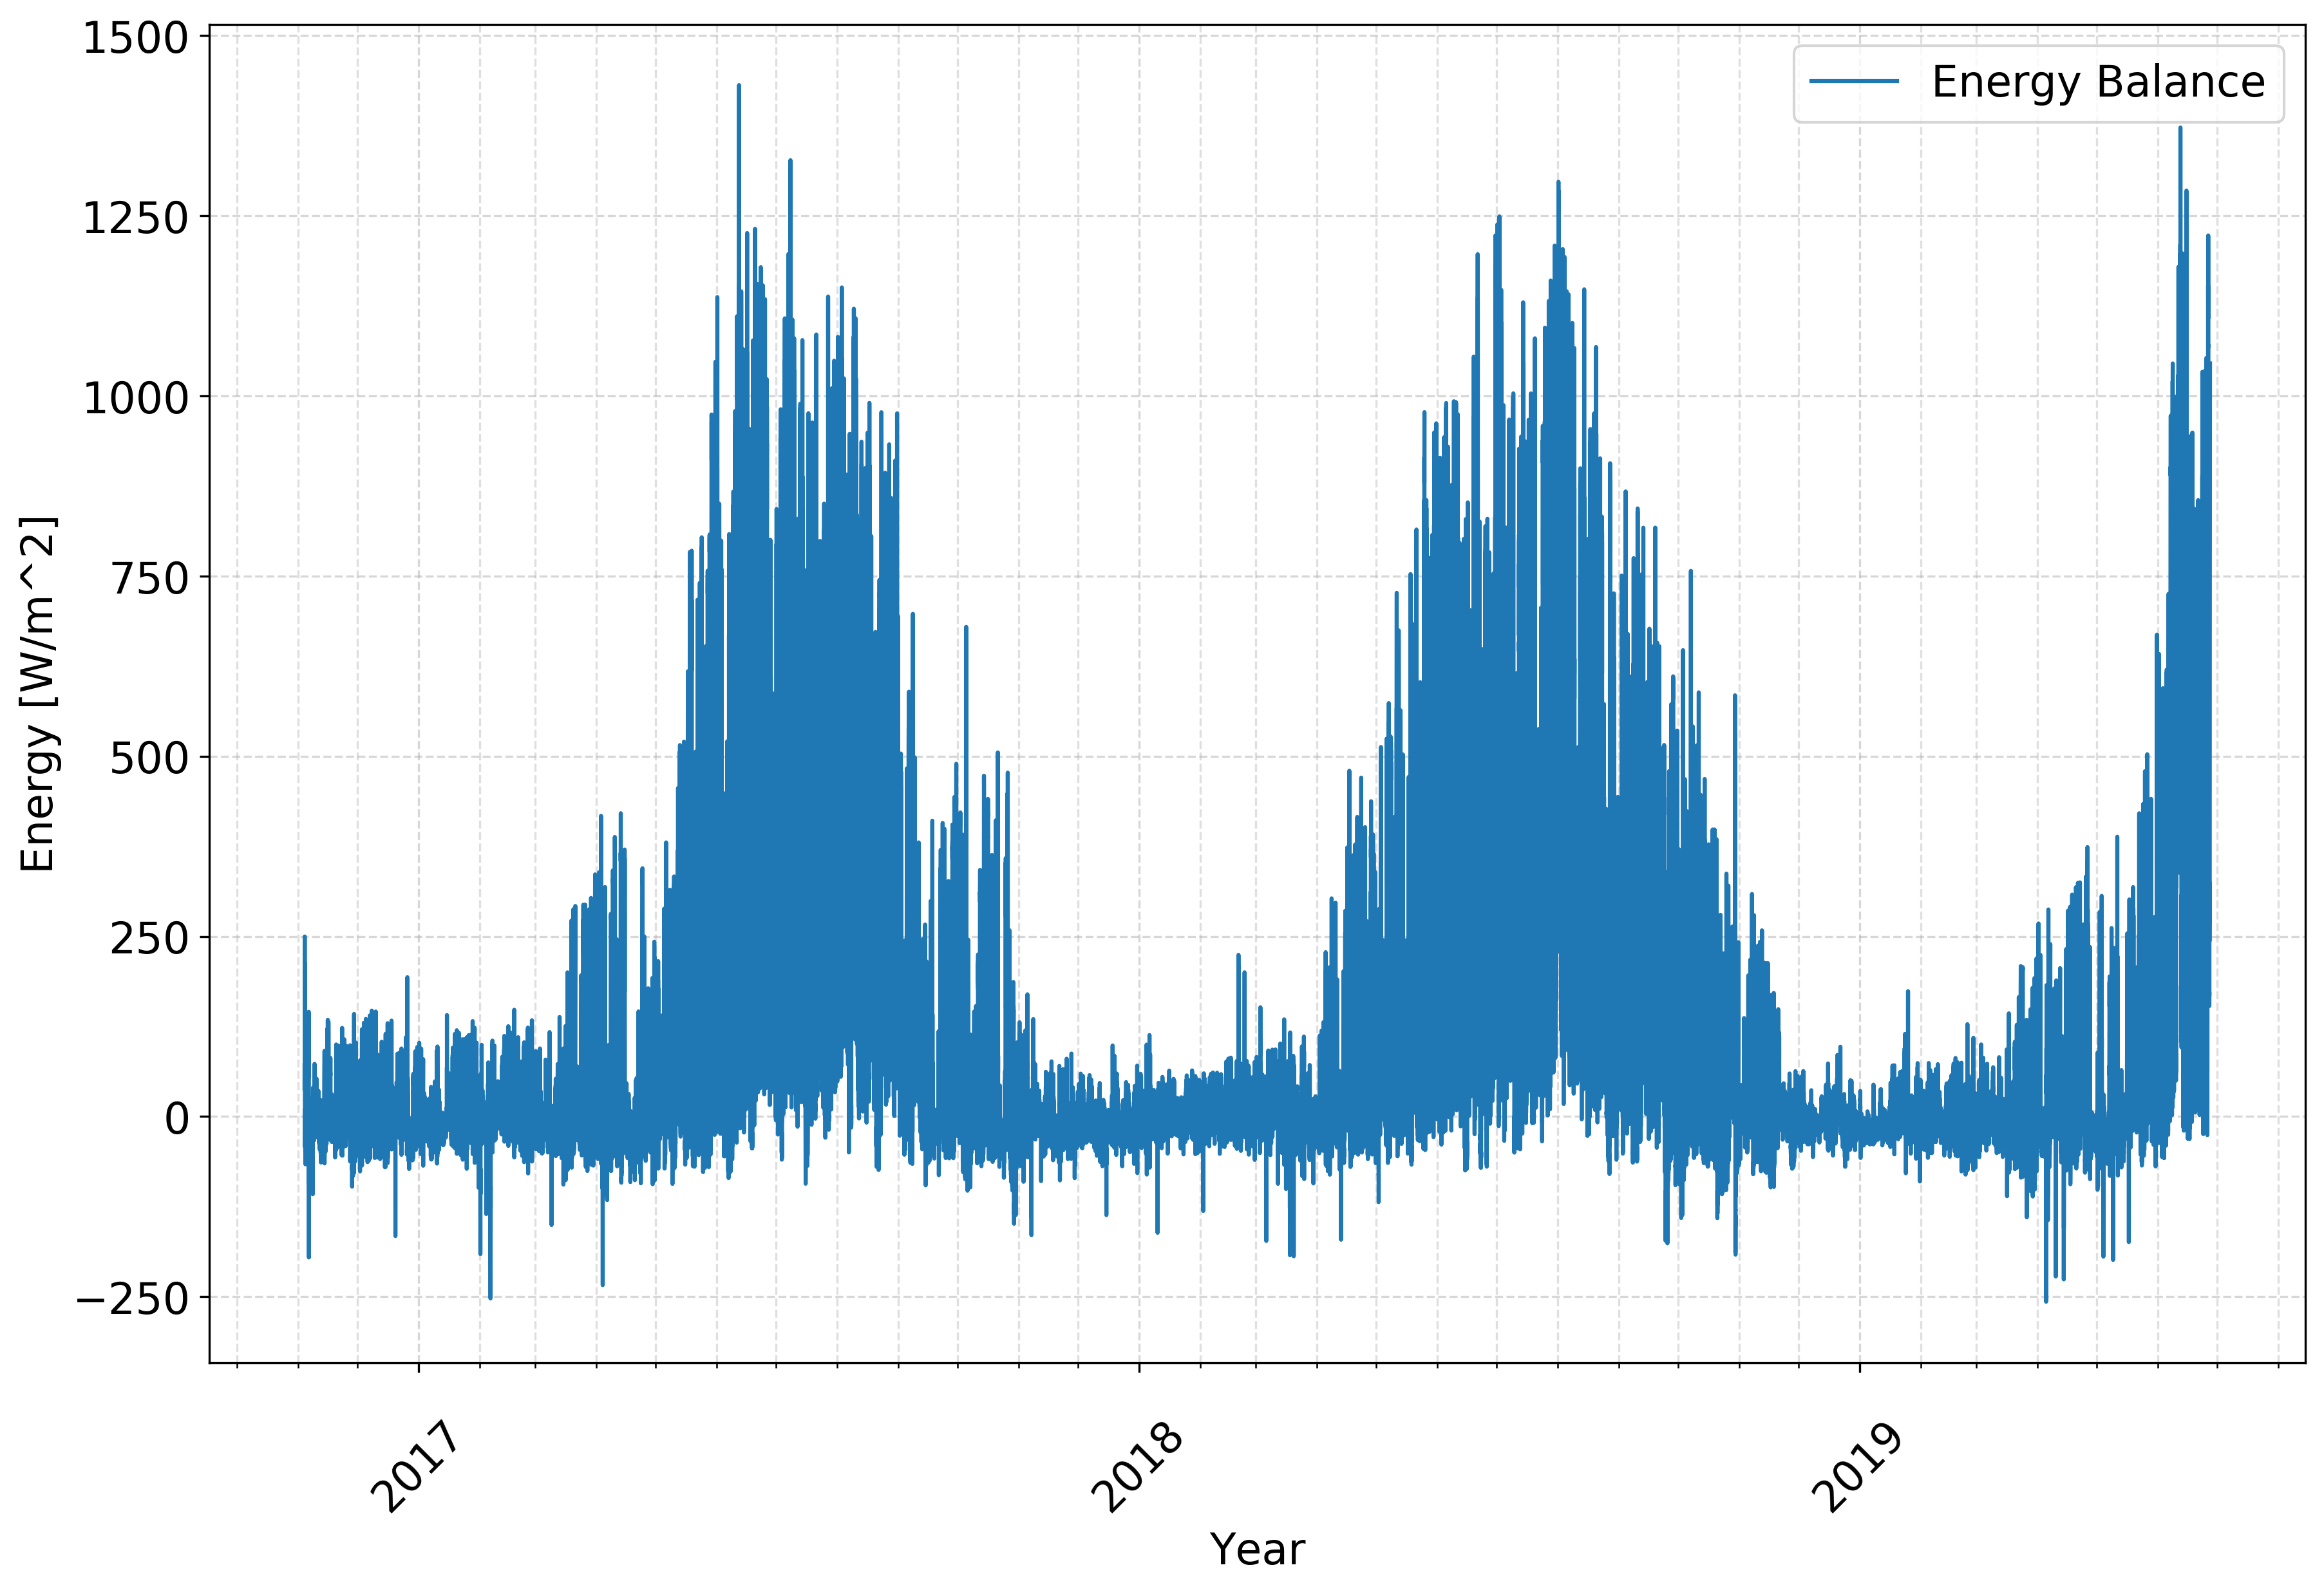
\includegraphics[width=1\textwidth]{../Software/plots/Total_energy_balance.png}
\caption{Energiebilanz gesamter Messzeitraum}
\label{fig:Energiebilanz gesamter Messzeitraum}
\end{figure}

Es sind leider nur knapp drei Jahre ausreichend Messdaten zur Berechnung der Energiebilanz verfügbar. An den Daten ist deutlich ein periodischer Verlauf erkennbar mit Maximum im Sommer und Minimum im Winter. Die Spitzen der Energiebilanz liegen bei knapp 1500 $W/m^2$, die Minima bei ca $-250 W/m^2$. Diese ungleiche Verteilung ist erklärbar durch die Messungen im Ablationsgebiet des Gletschers. Hier sollte ja das Jahresmittel deutlich positiv sein. Folgende Tabelle zeigt die zwei Mittelwerte der Energiebilanz in den Jahren 2017 und 2018.

TABELLE MITTEL 
EB mean 2017 100.4 %W/m^2
EB mean 2018 109.1 %W/m^2

Die nachfolgende Abbildung zeigt den gleichen Zusammenhang wie zuvor, jedoch wurden hier jeweils zwei Tage gemittelt.

\begin{figure}[H]
\centering
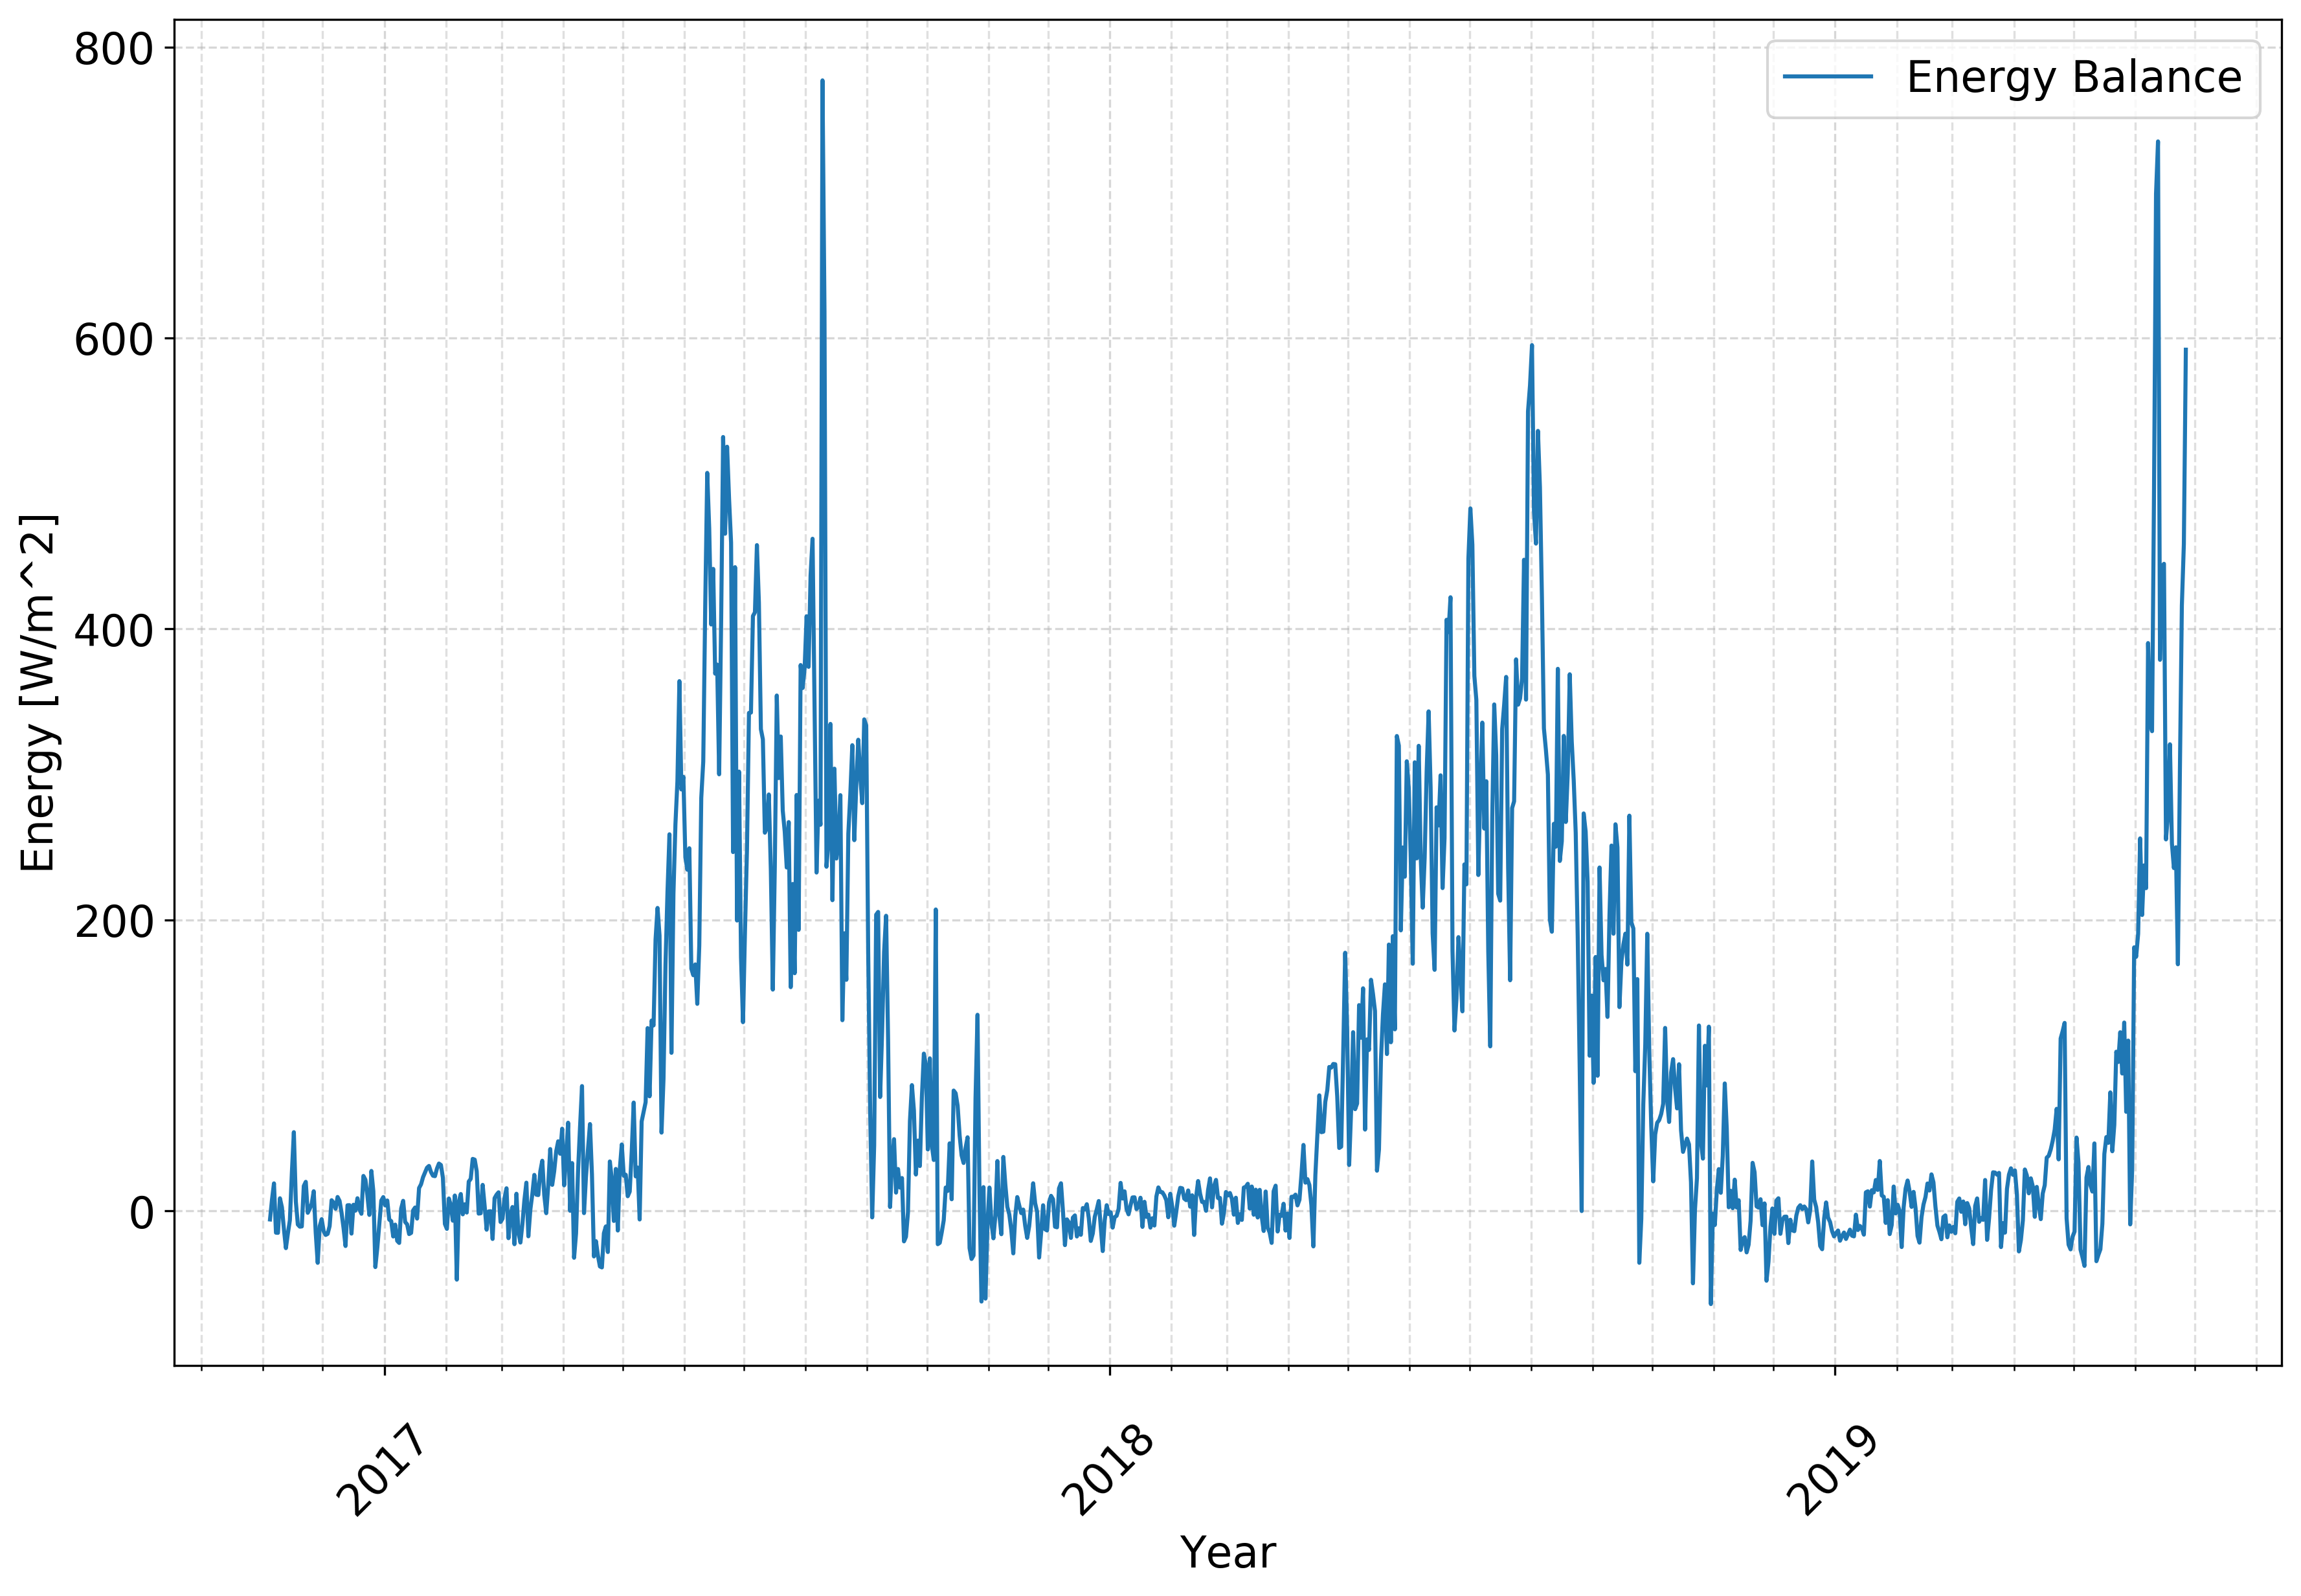
\includegraphics[width=1\textwidth]{../Software/plots/Total_energy_balance_summed.png}
\caption{Energiebilanz gesamter Messzeitraum 2 tägiges Mittel}
\label{fig:..}
\end{figure}

 Dies resultiert in einem glatteren Verlauf der Kurve, wobei es im Bereich des Sommers zwischen unterschiedlichen 2-Tages-Werten trotzdem noch Abweichungen von teils 300 $W/m^2$ gibt. Dies lässt sich auf unterschiedliche Wetterlagen zurückführen und könnte gut mit Sonnenscheinzeiten pro Tag usw. verglichen werden.\\
Das Aufsummieren der Bilanzen bringt einen Ausreißer gegen Ende der Messreihe im Juni 2019 zum Vorschein. Dieses zweitätige Mittel von mehr als 700 $W/m^2$ ist mit knapp 200 $W/m^2$ Vorsprung der größe Wert im betrachteten Zeitraum. Durch Darstellung von einzelnen Komponenten der Energiebilanz kann erörtert werden, woraus dieser Maximalwert hervorgeht.\\

Abbildung \ref{fig:Strahlungskomponente im gesamten Messzeitraum} zeigt die kombinierten Bestandteile ``Short wave in'', ``Short wave out'', ``Long wave in'' und ``Long wave out''

\begin{figure}[H]
\centering
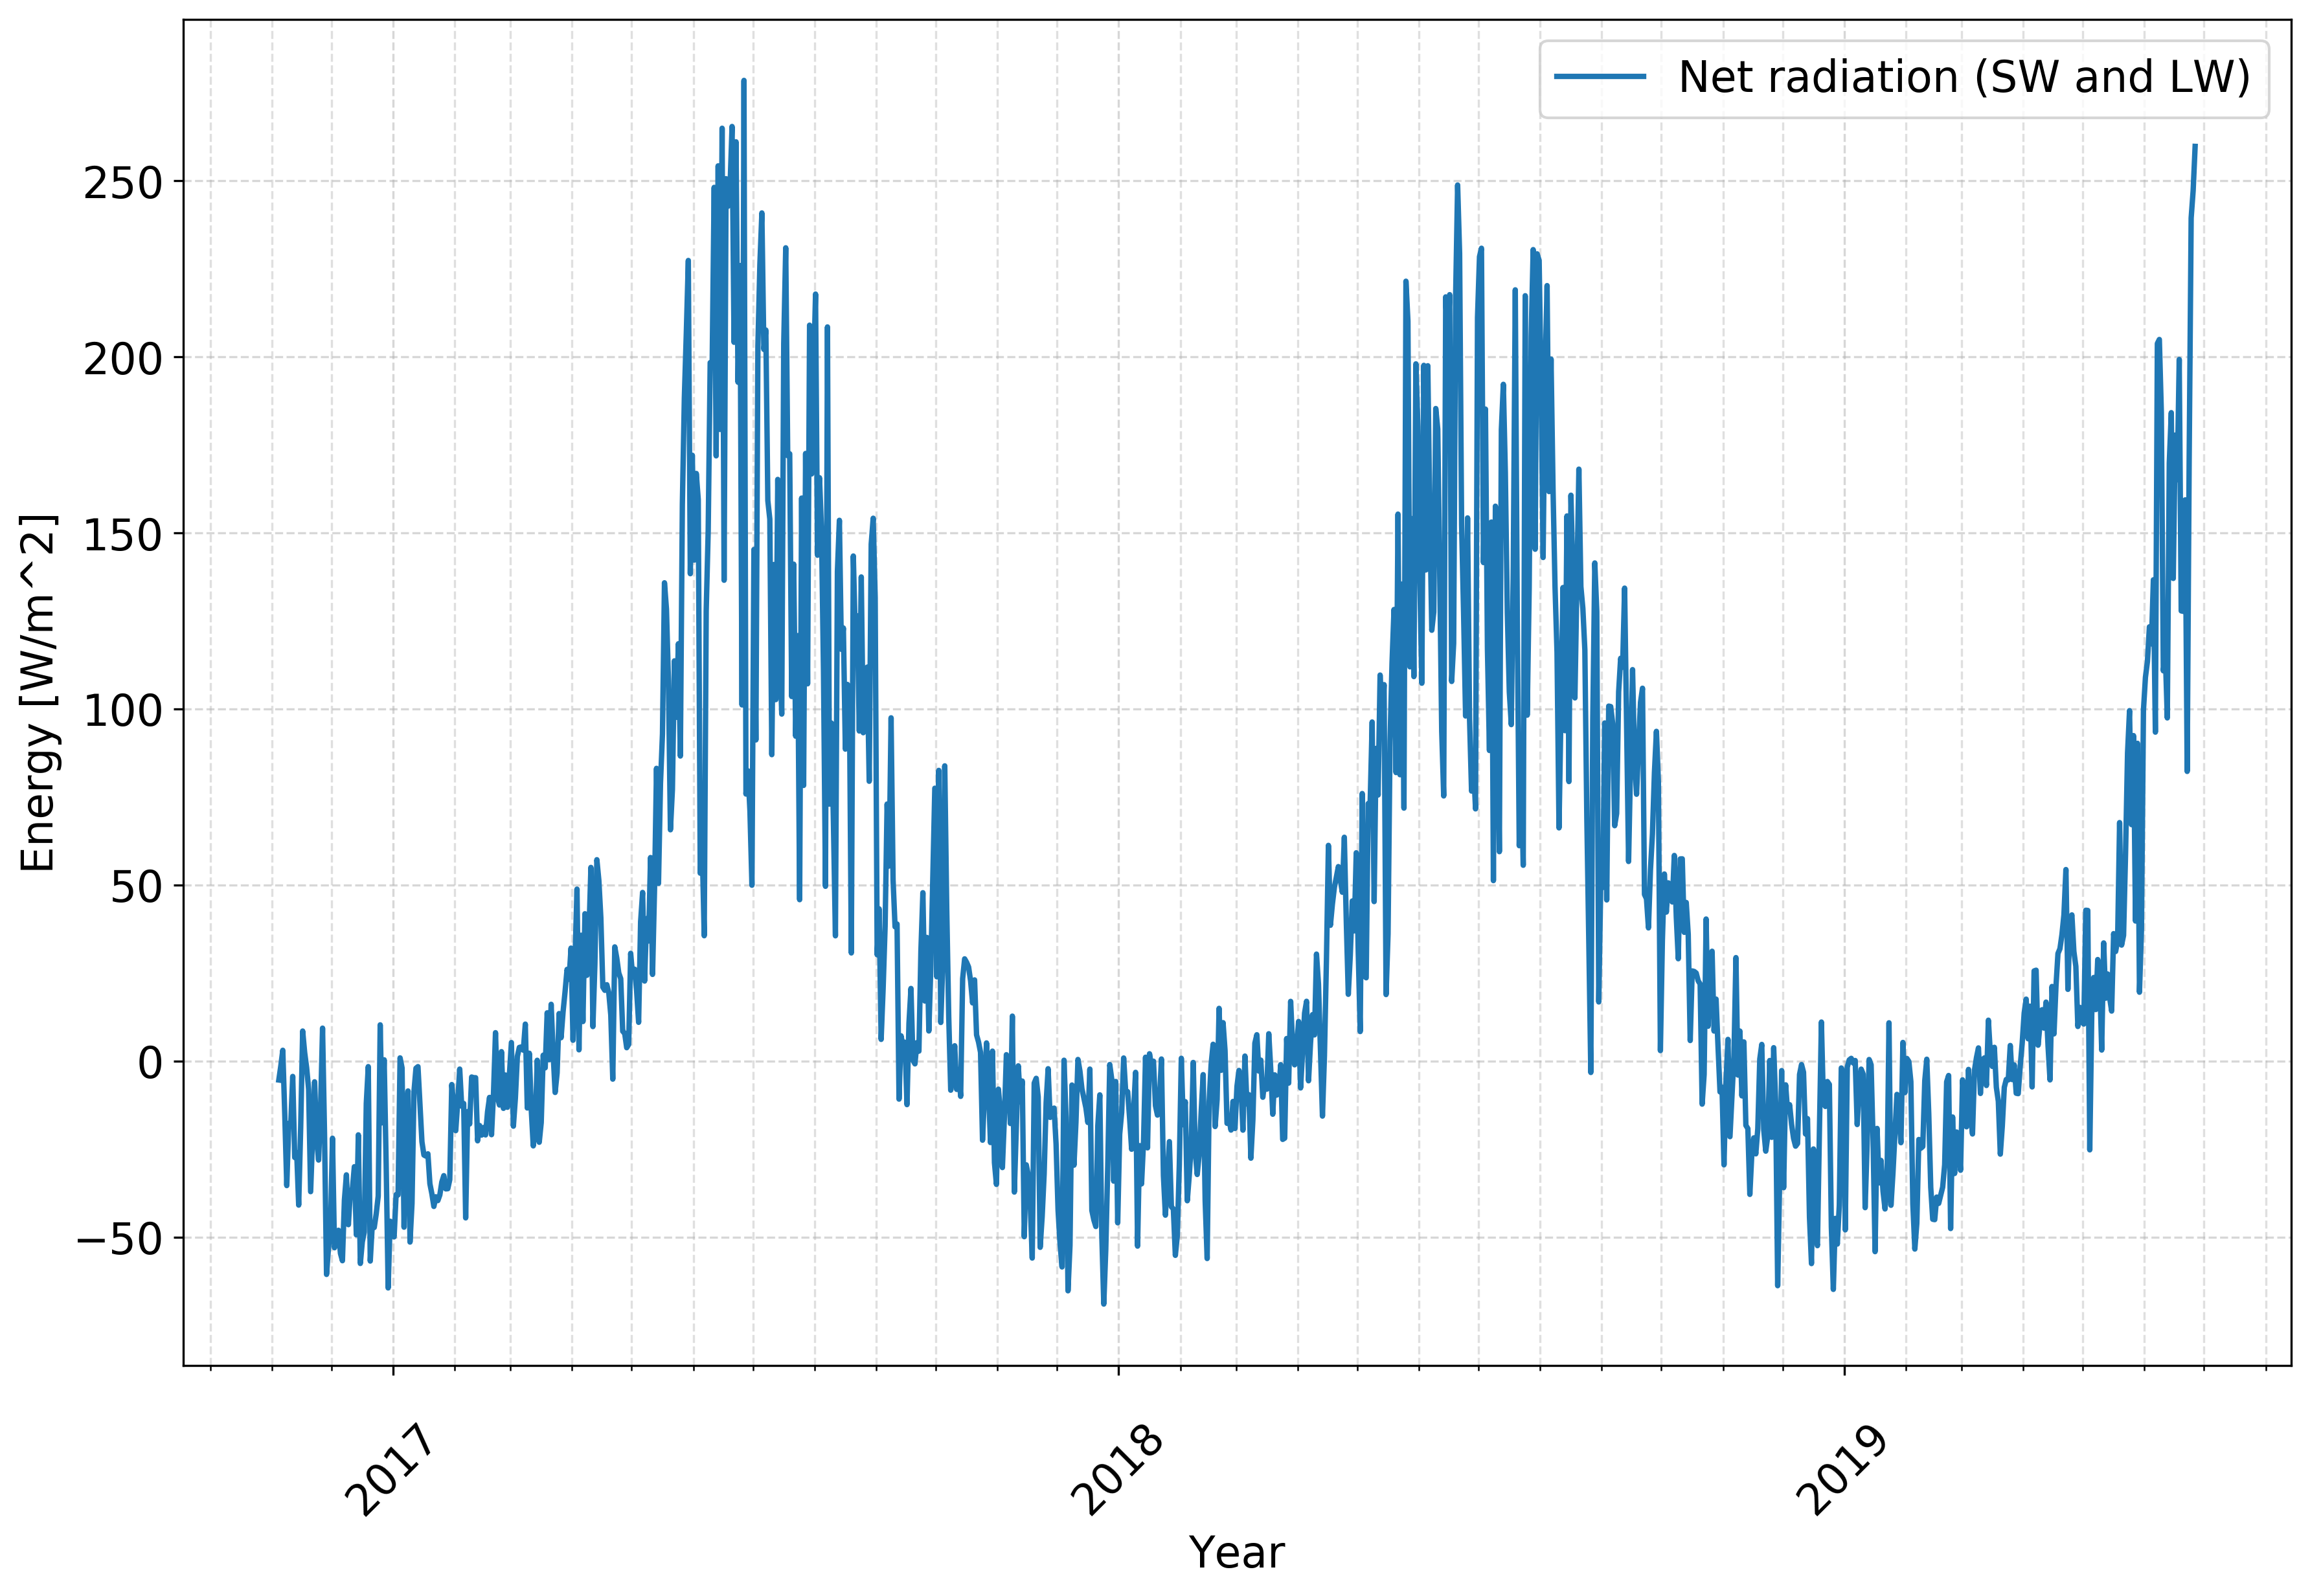
\includegraphics[width=1\textwidth]{../Software/plots/Energy_balance_only_radiation.png}
\caption{Strahlungskomponente im gesamten Messzeitraum}
\label{fig:Strahlungskomponente im gesamten Messzeitraum}
\end{figure}


\begin{figure}[H]
\centering
\includegraphics[width=1\textwidth]{../Software/plots/Energy_balance_only_sens_and_latent_heat.png}
\caption{Kompletter Zeitraum aufsummiert nur sensible und latent heat}
\label{fig:..}
\end{figure}

\begin{figure}[H]
\centering
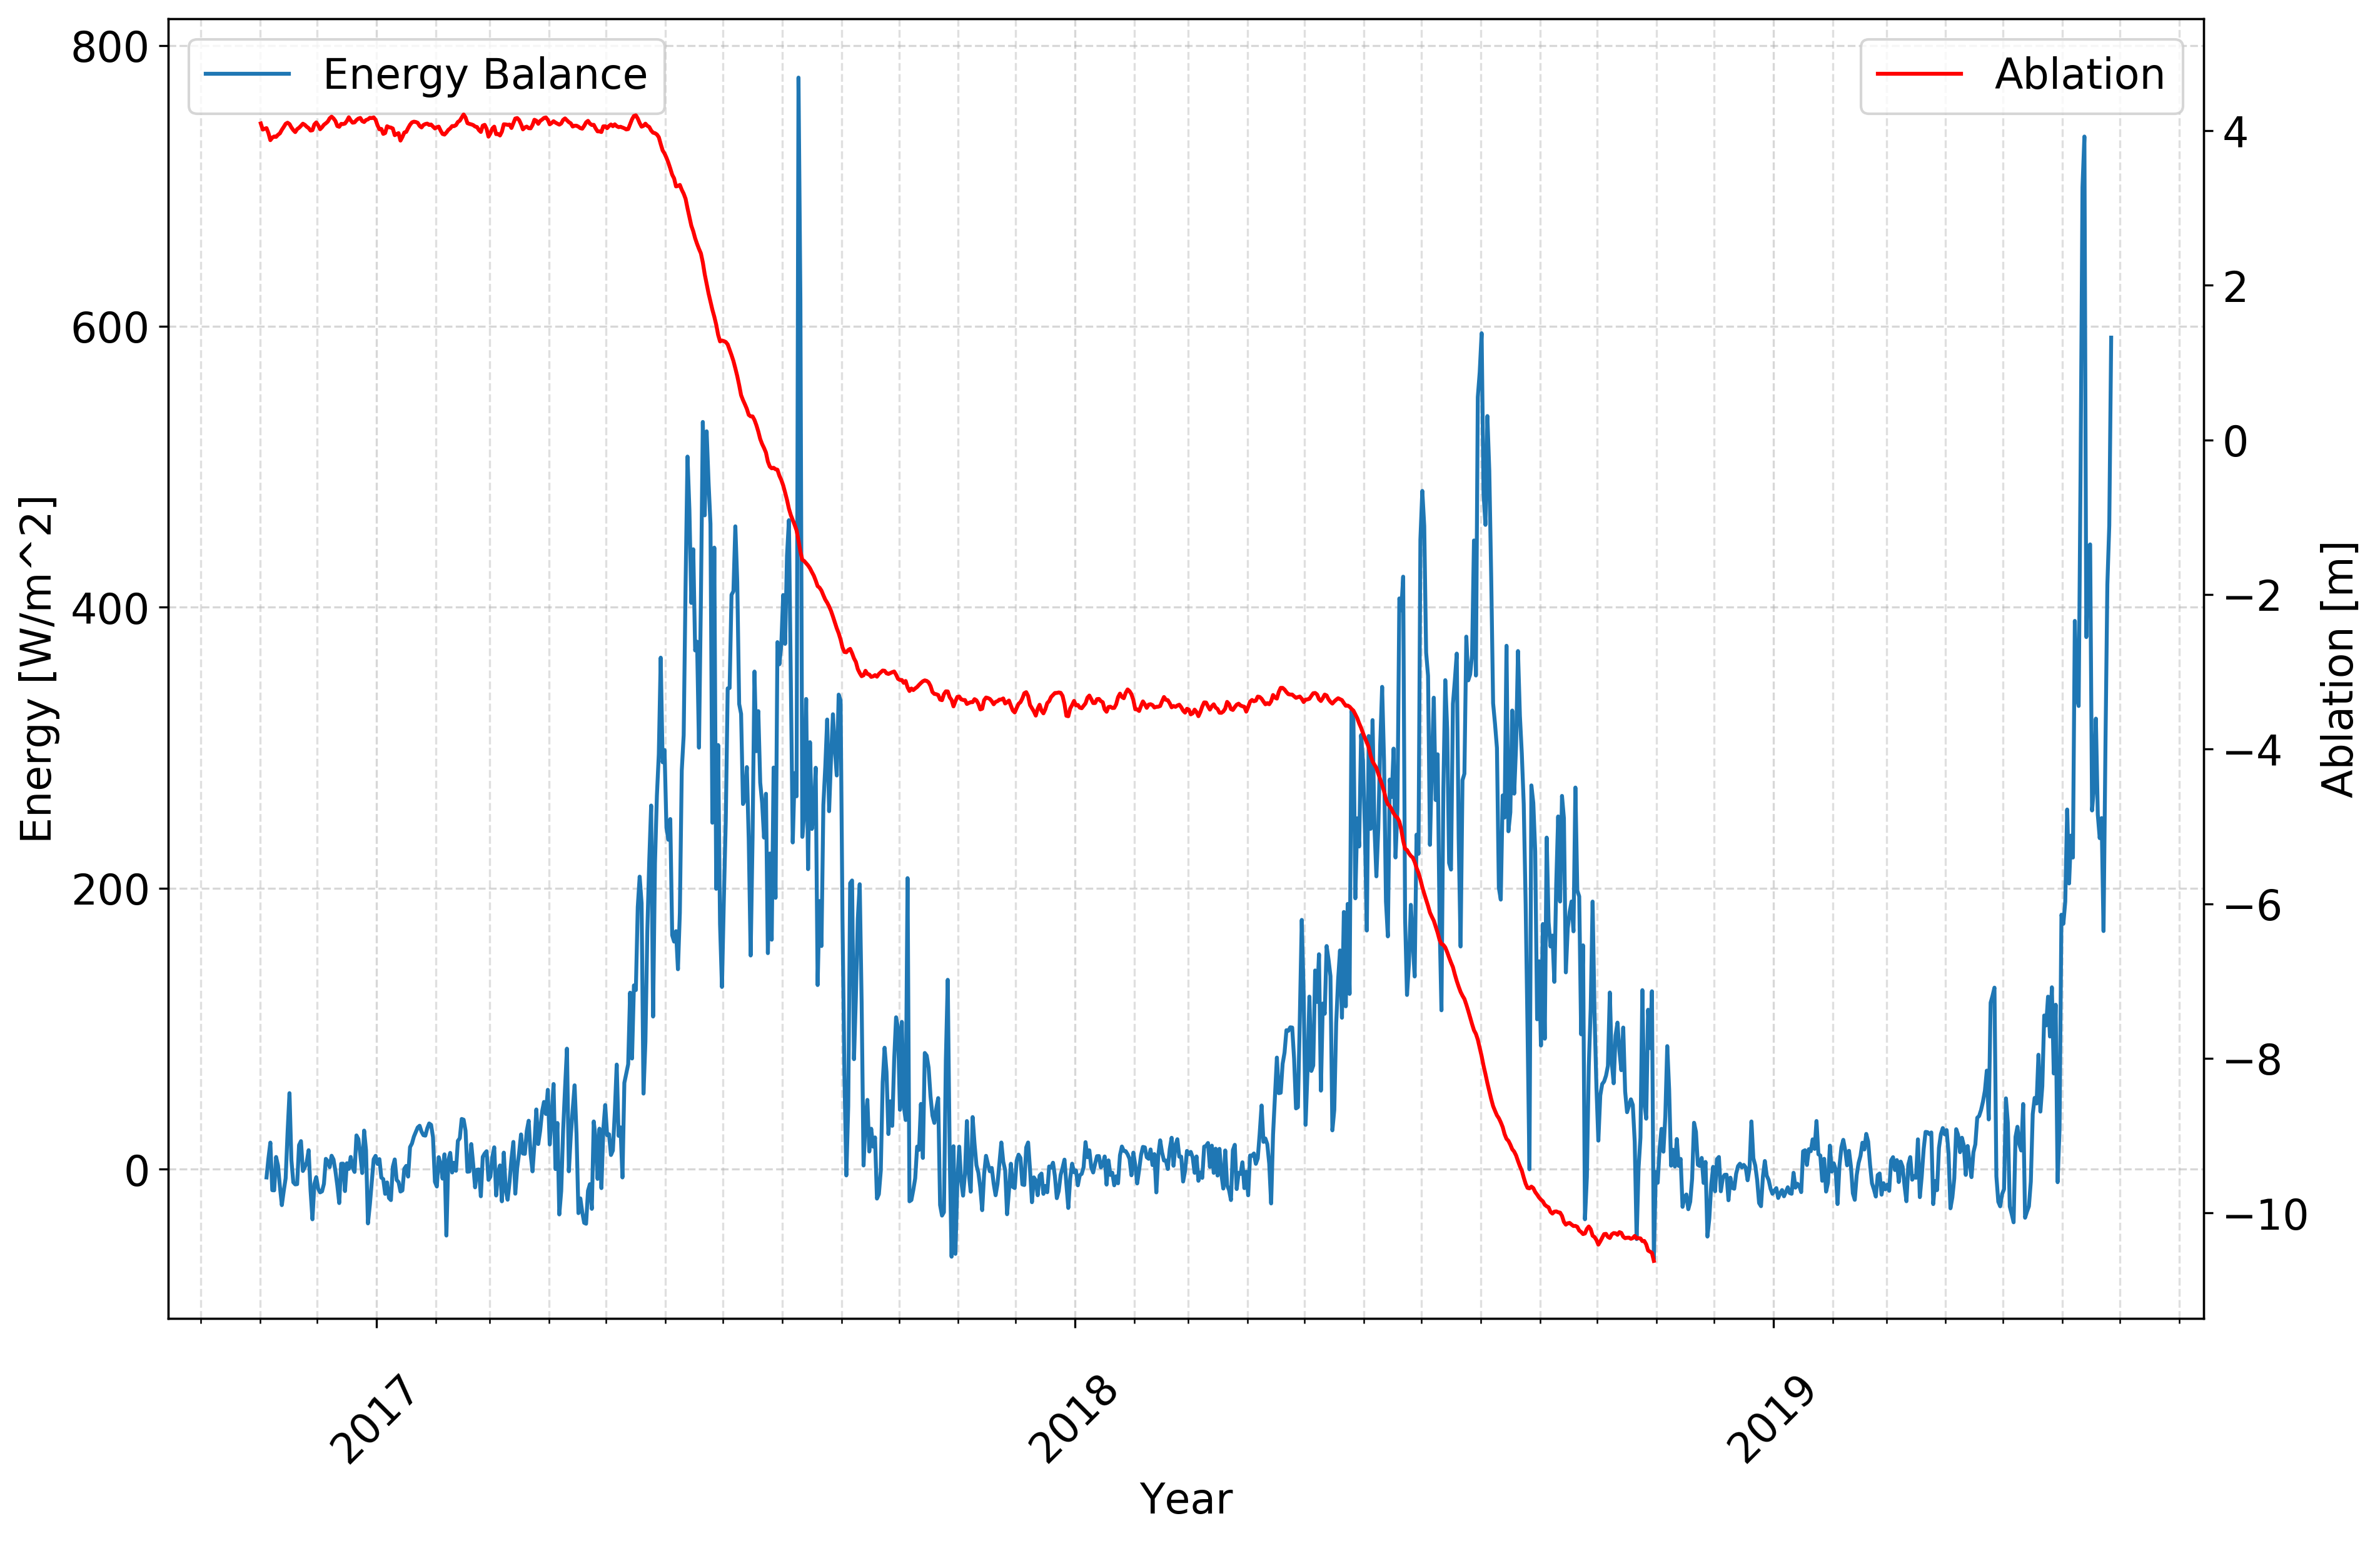
\includegraphics[width=1\textwidth]{../Software/plots/Total_energy_balance_summed_with_ablation.png}
\caption{Kompletter Zeitraum aufsummiert nur sensible und latent heat}
\label{fig:..}
\end{figure}


\begin{figure}[H]
\centering
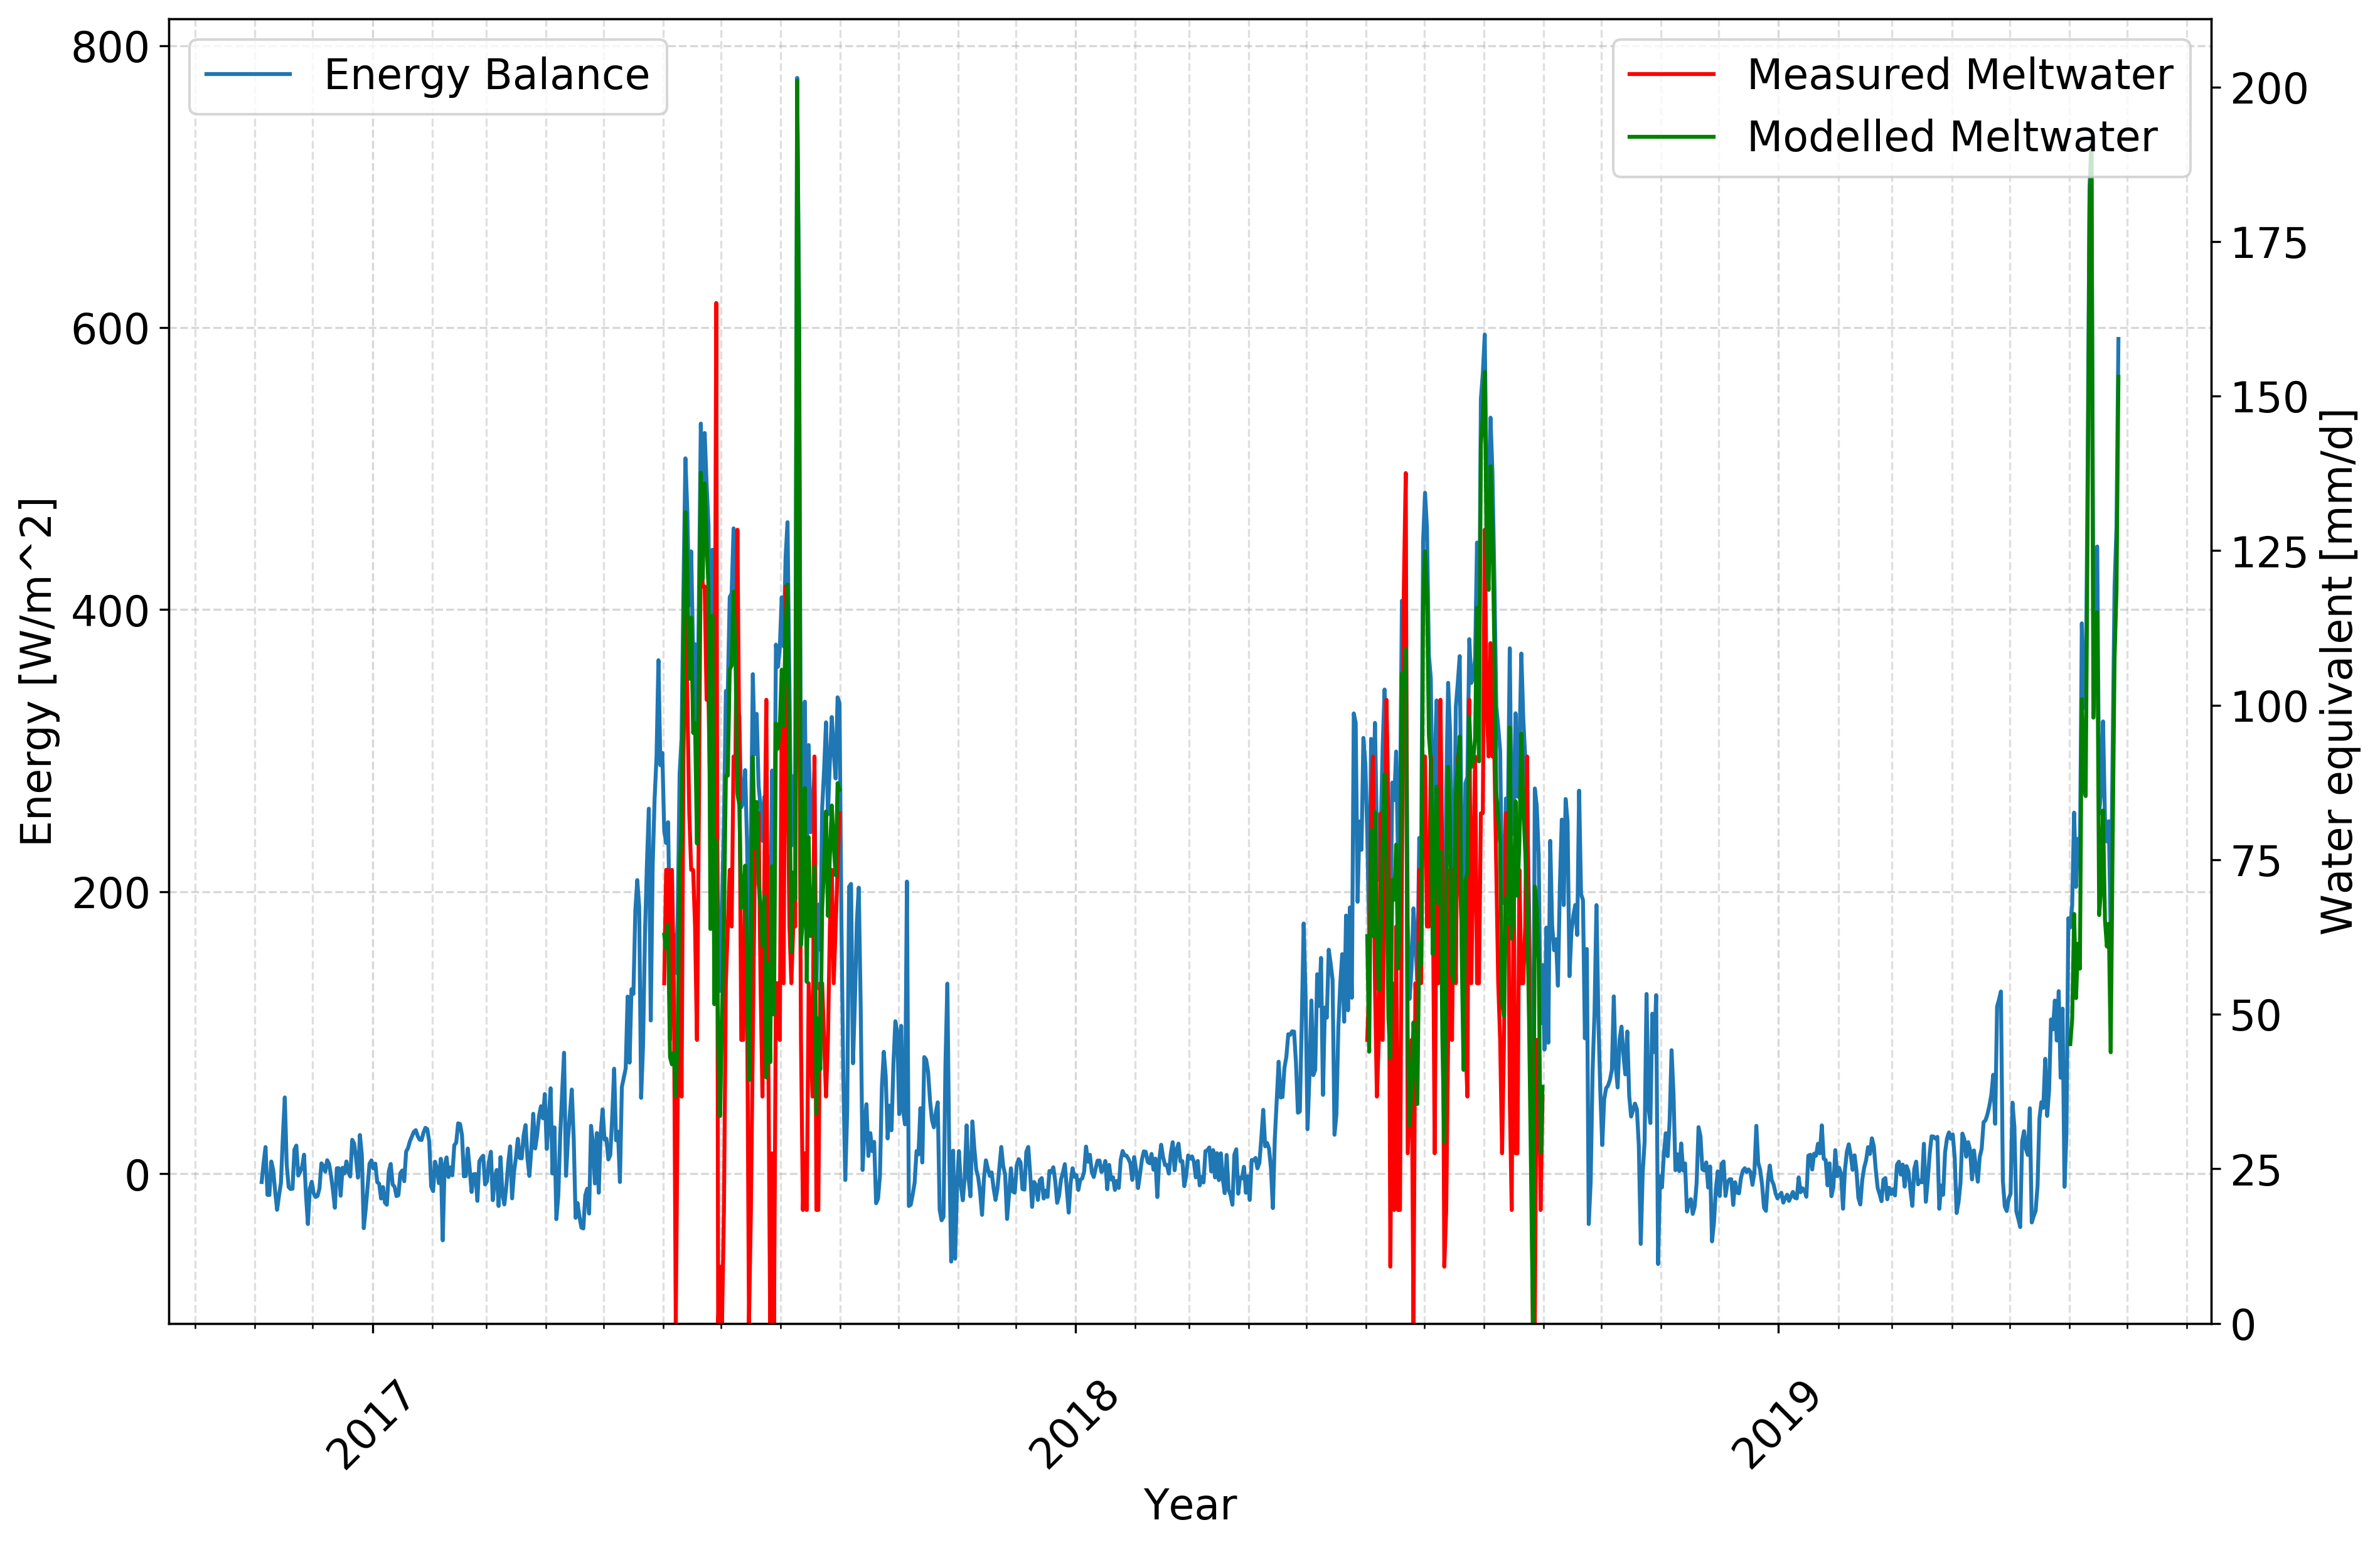
\includegraphics[width=1\textwidth]{../Software/plots/Total_energy_balance_summed_with_water_equivalent.png}
\caption{Kompletter Zeitraum aufsummiert nur sensible und latent heat}
\label{fig:..}
\end{figure}


\begin{figure}[H]
\centering
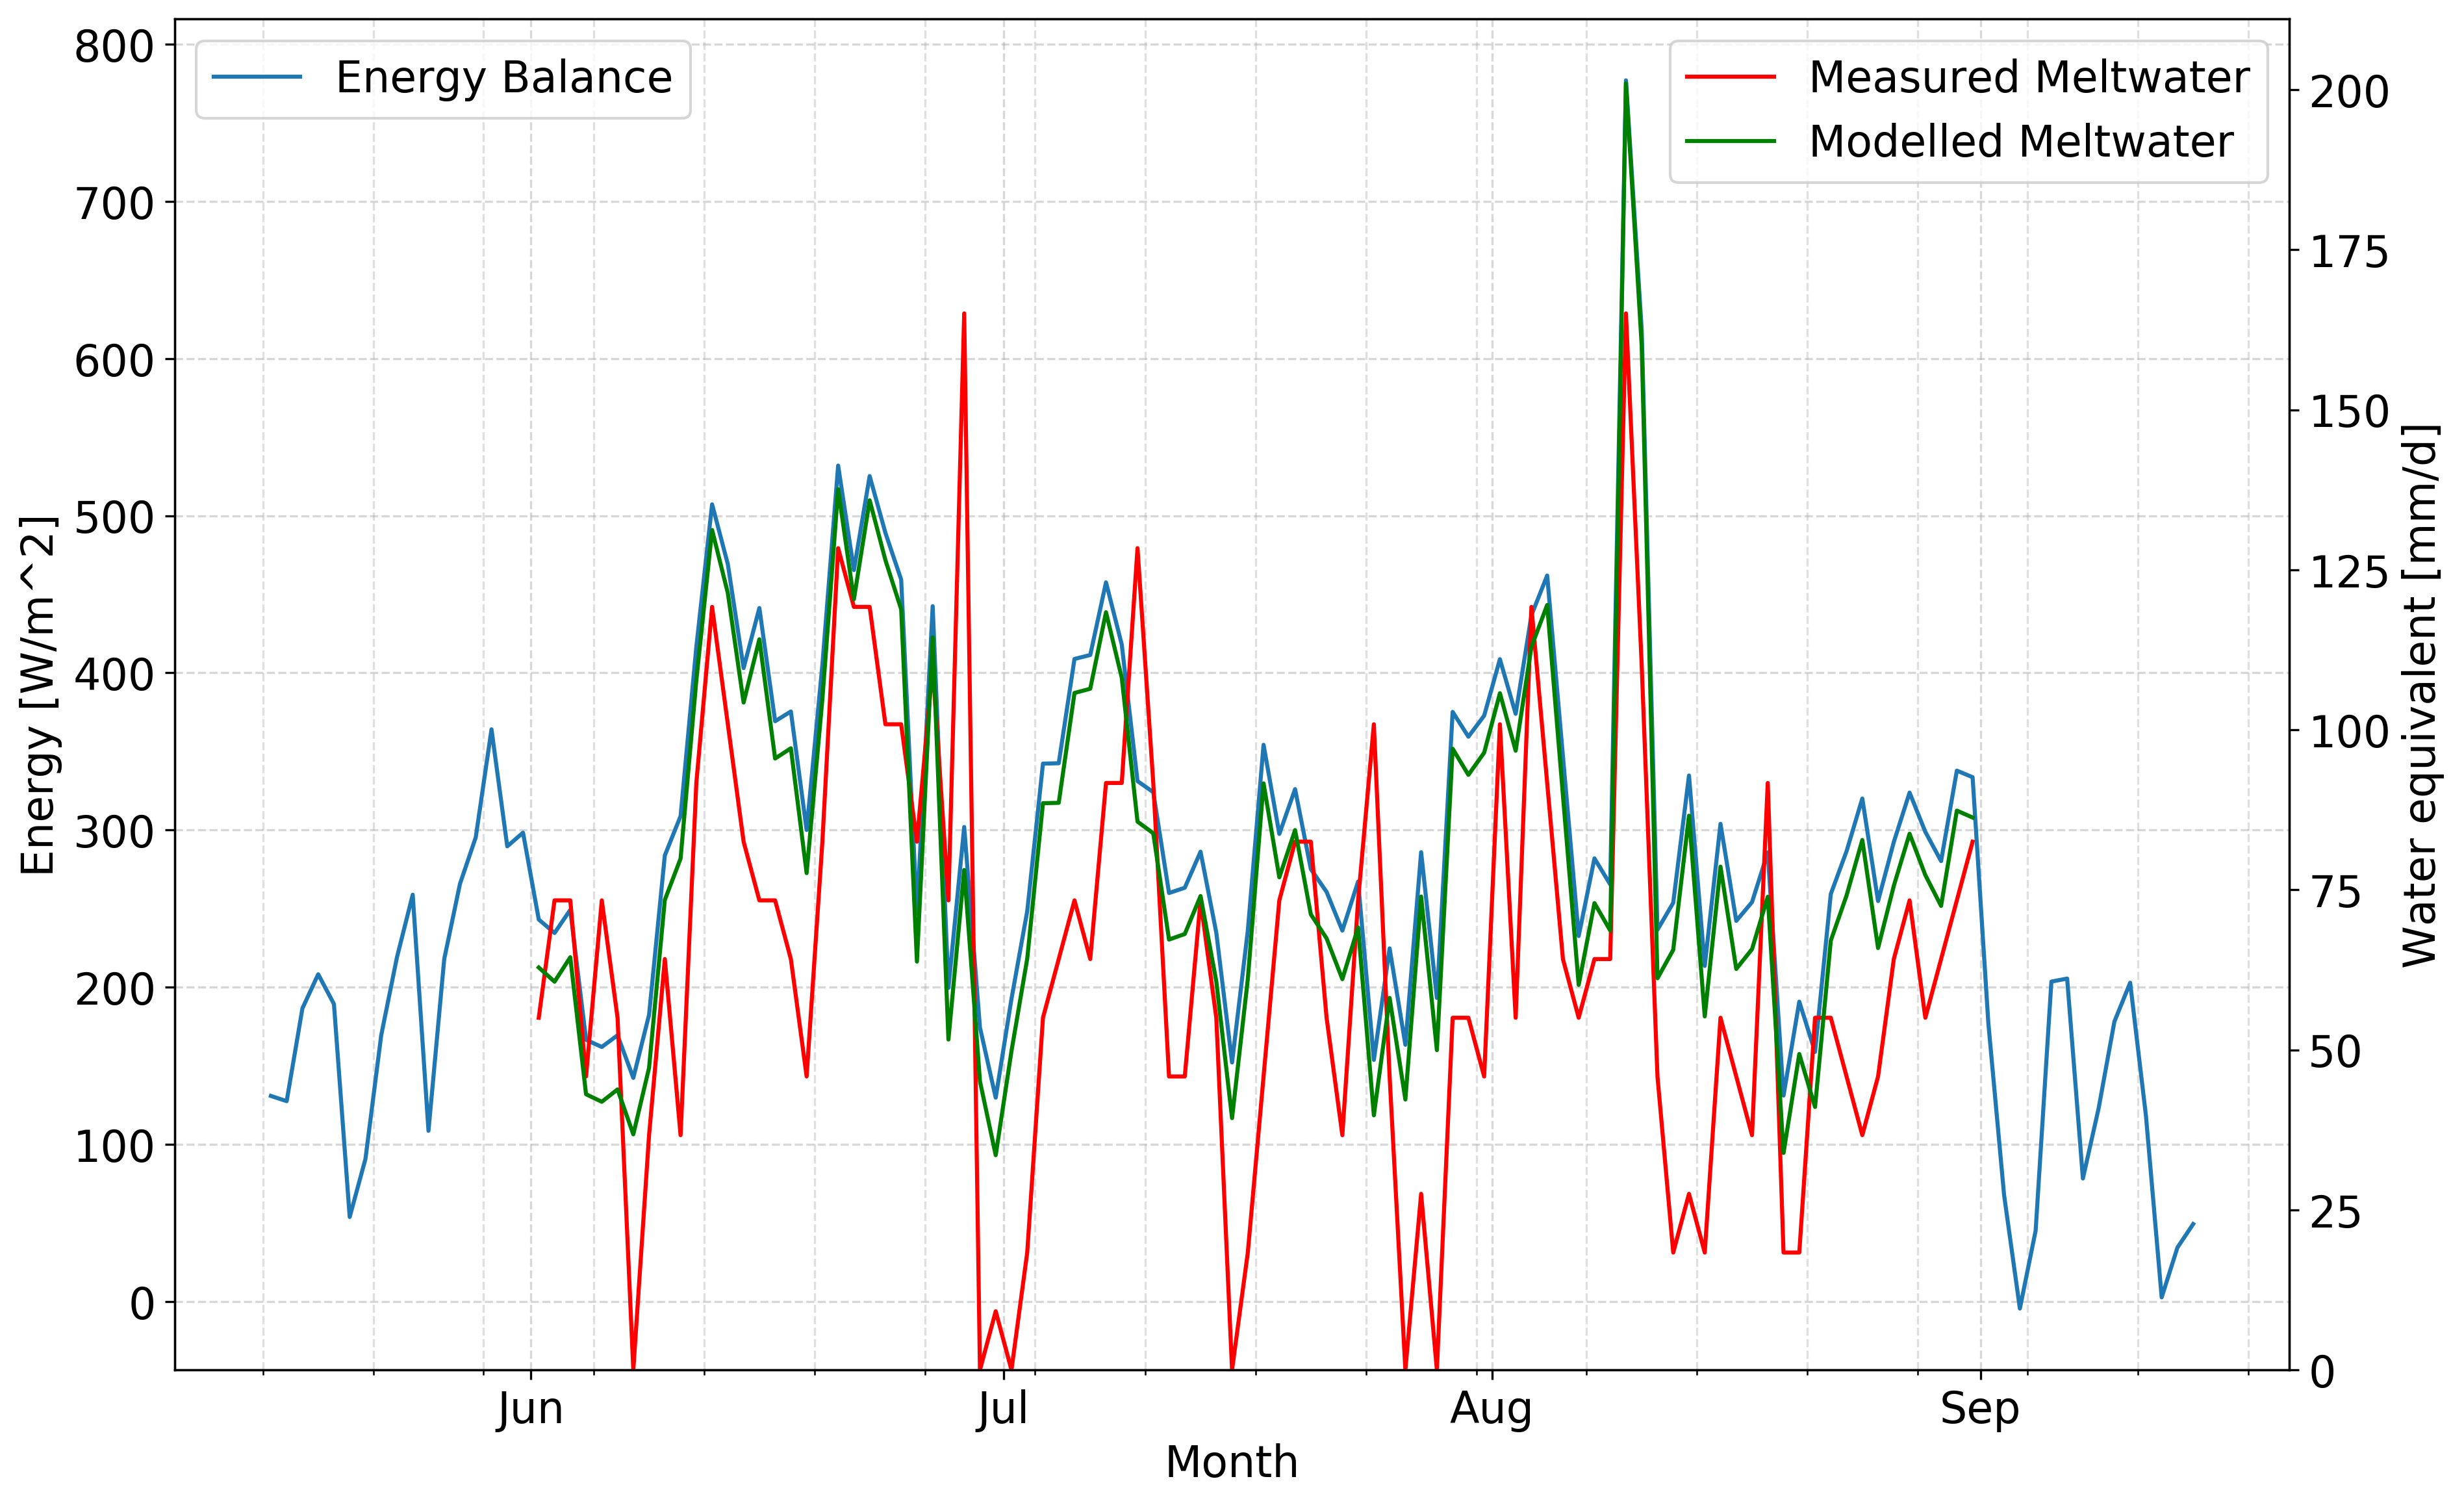
\includegraphics[width=1\textwidth]{../Software/plots/Total_energy_balance_summed_with_water_equivalent_2017.png}
\caption{Kompletter Zeitraum aufsummiert nur sensible und latent heat}
\label{fig:..}
\end{figure}

\begin{figure}[H]
\centering
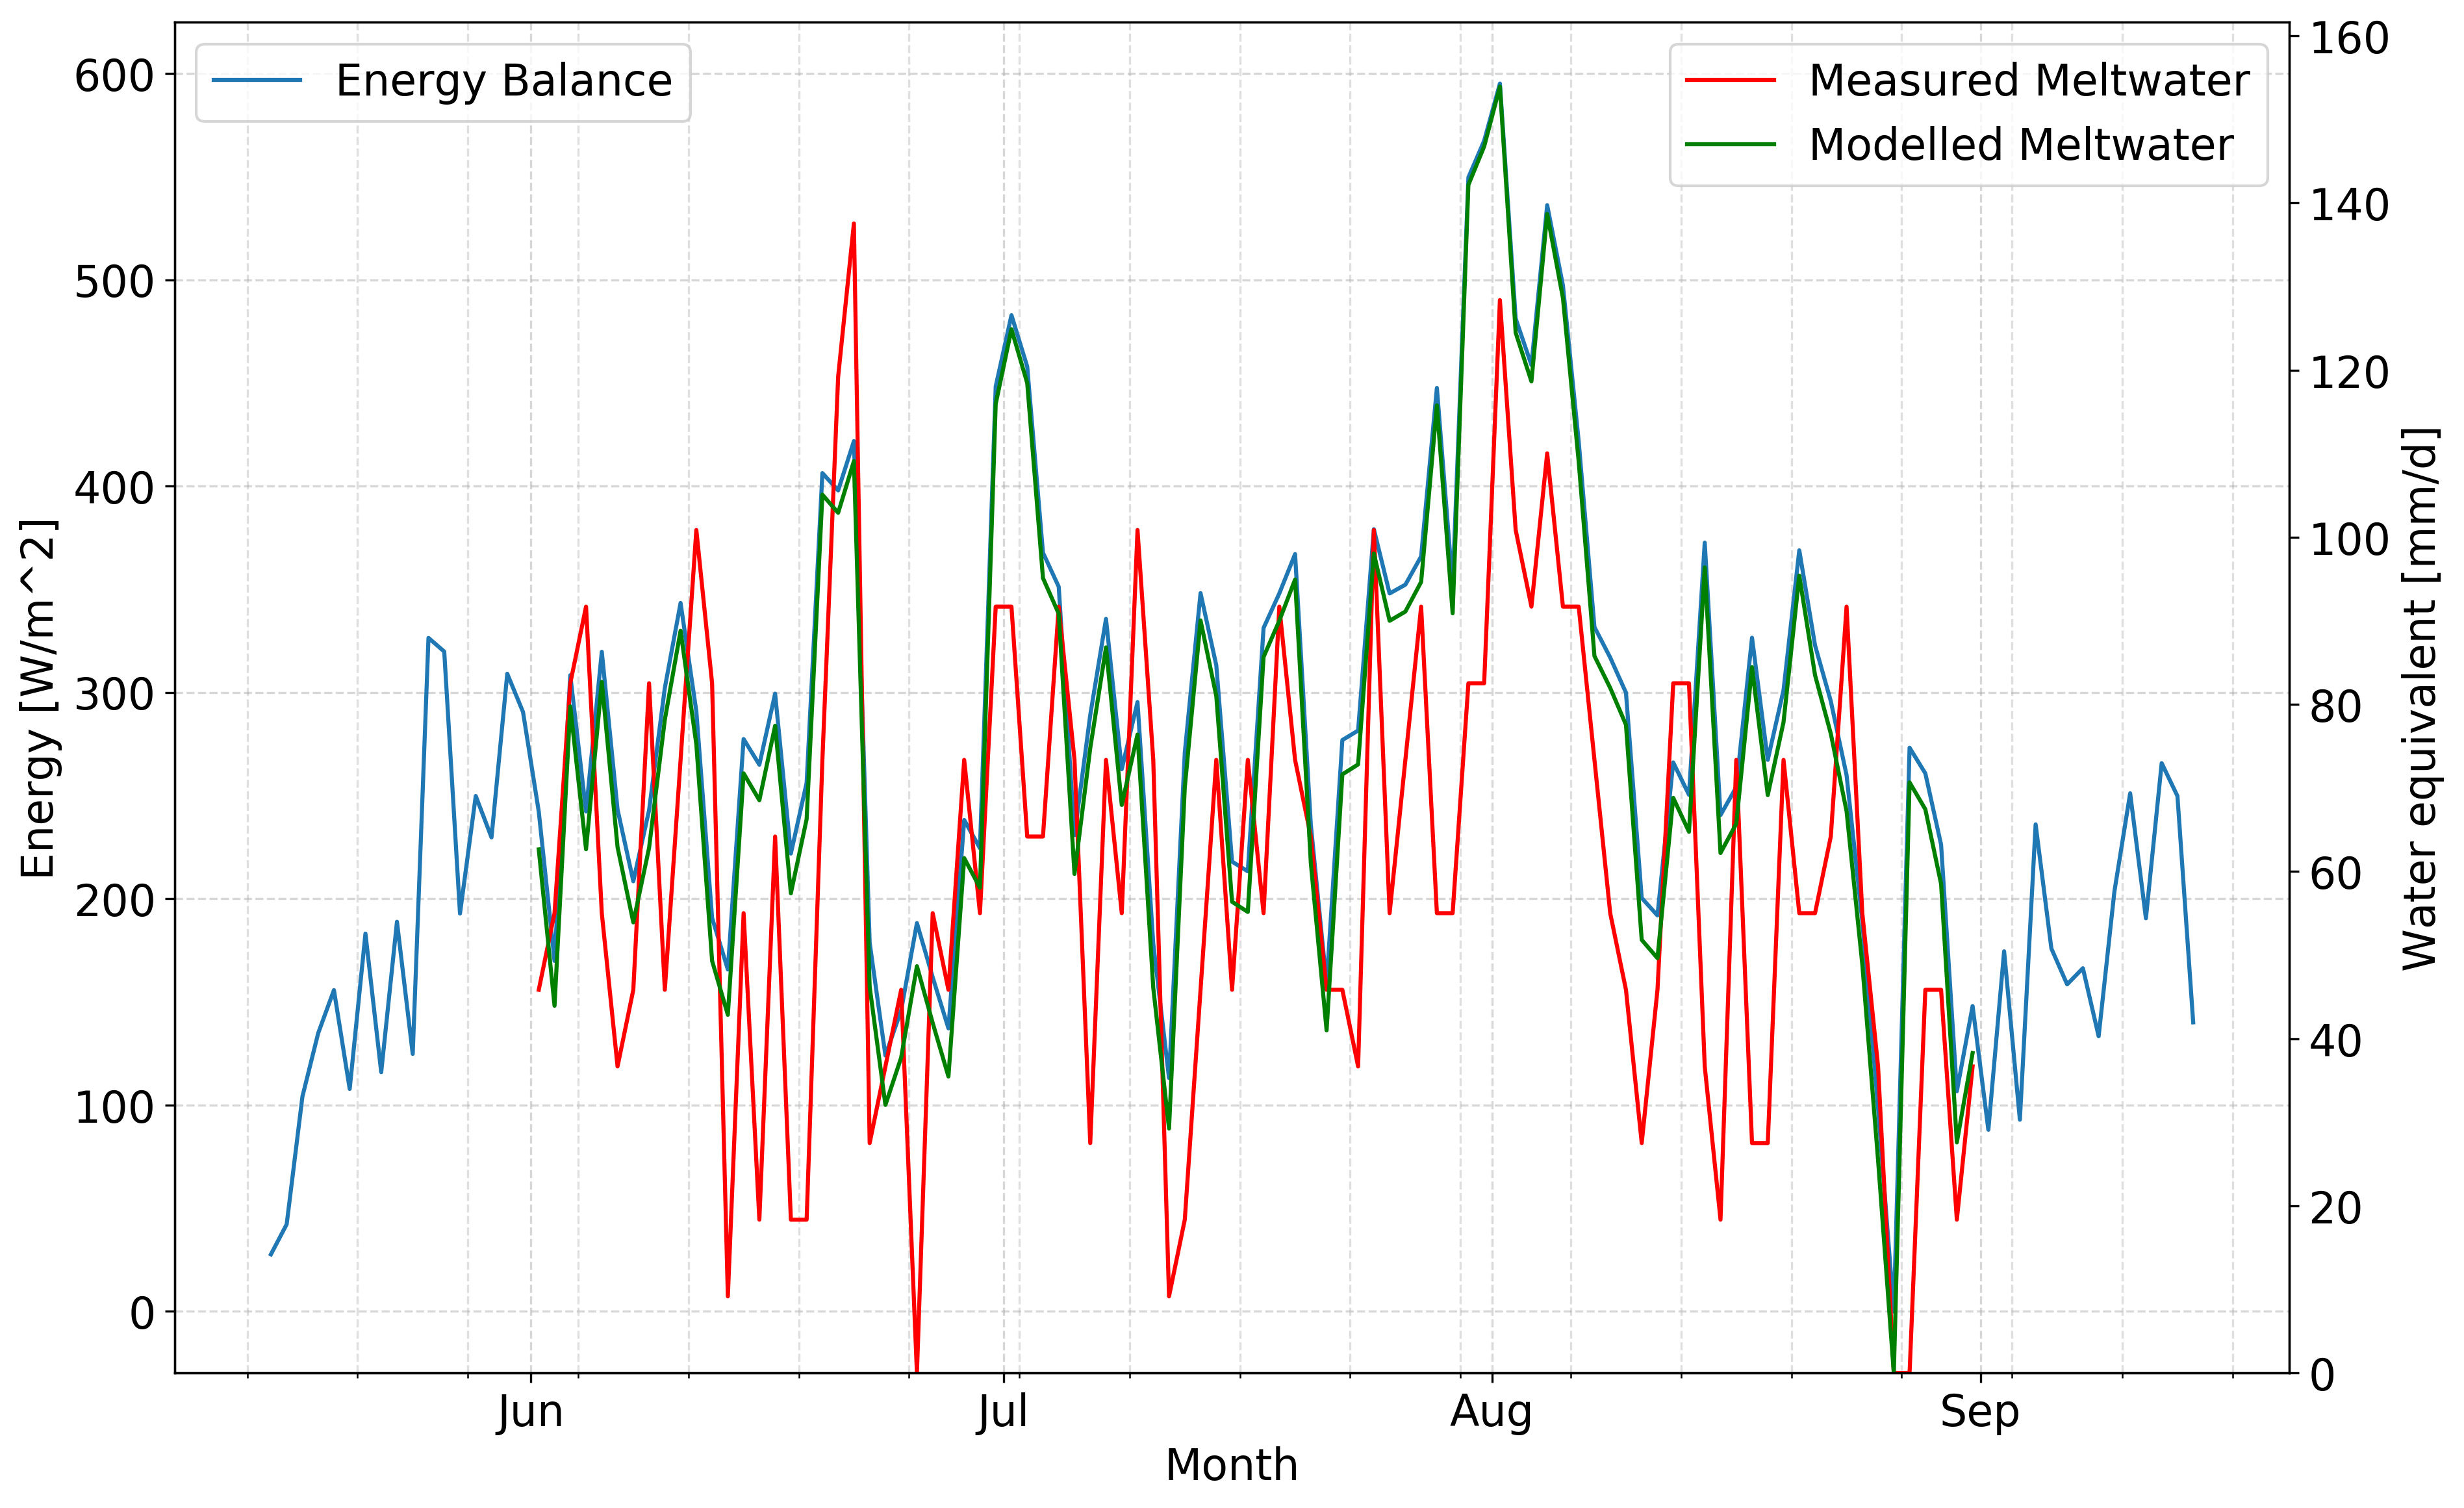
\includegraphics[width=1\textwidth]{../Software/plots/Total_energy_balance_summed_with_water_equivalent_2018.png}
\caption{Kompletter Zeitraum aufsummiert nur sensible und latent heat}
\label{fig:..}
\end{figure}


Bei sehr Ablaiton 0 oder größer 0 wird 0 als Schmelzwasser angenommen  .. deshalb die Spitzen nach unten?

\begin{figure}[H]
\centering
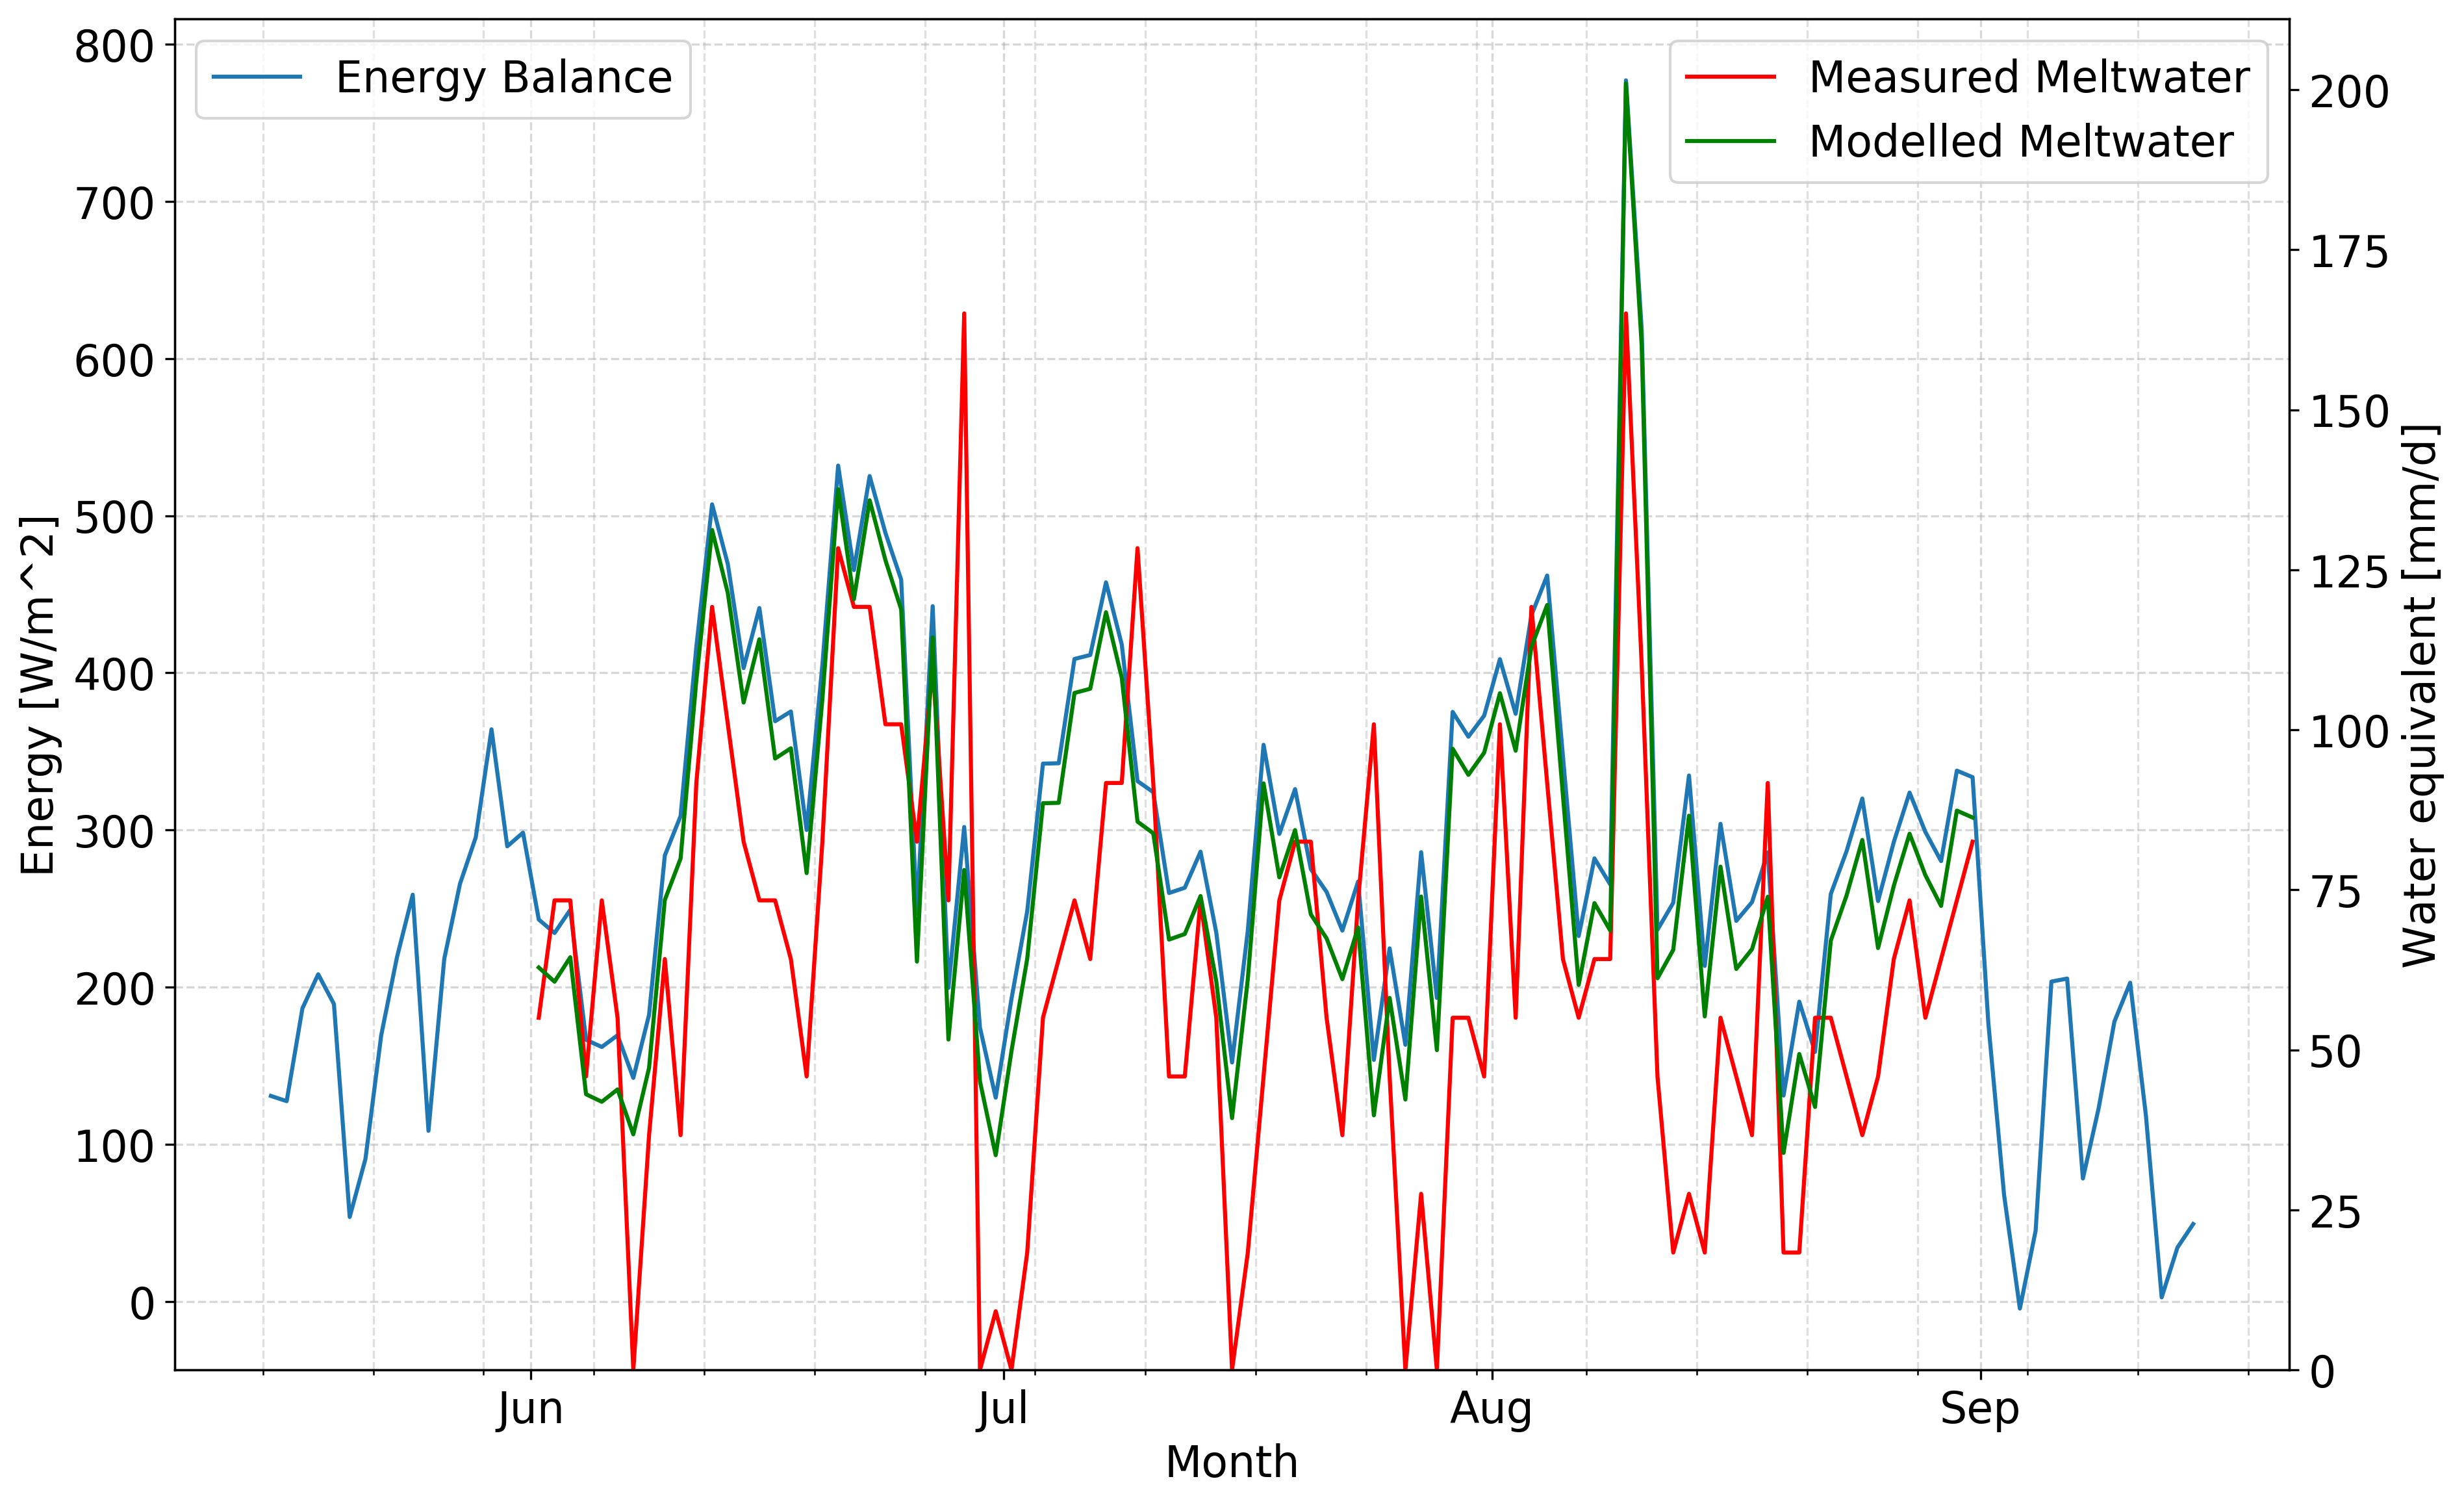
\includegraphics[width=1\textwidth]{../Software/plots/Total_energy_balance_summed_with_water_equivalent_2017.png}
\caption{Kompletter Zeitraum aufsummiert nur sensible und latent heat}
\label{fig:..}
\end{figure}




\begin{figure}[H]
\centering
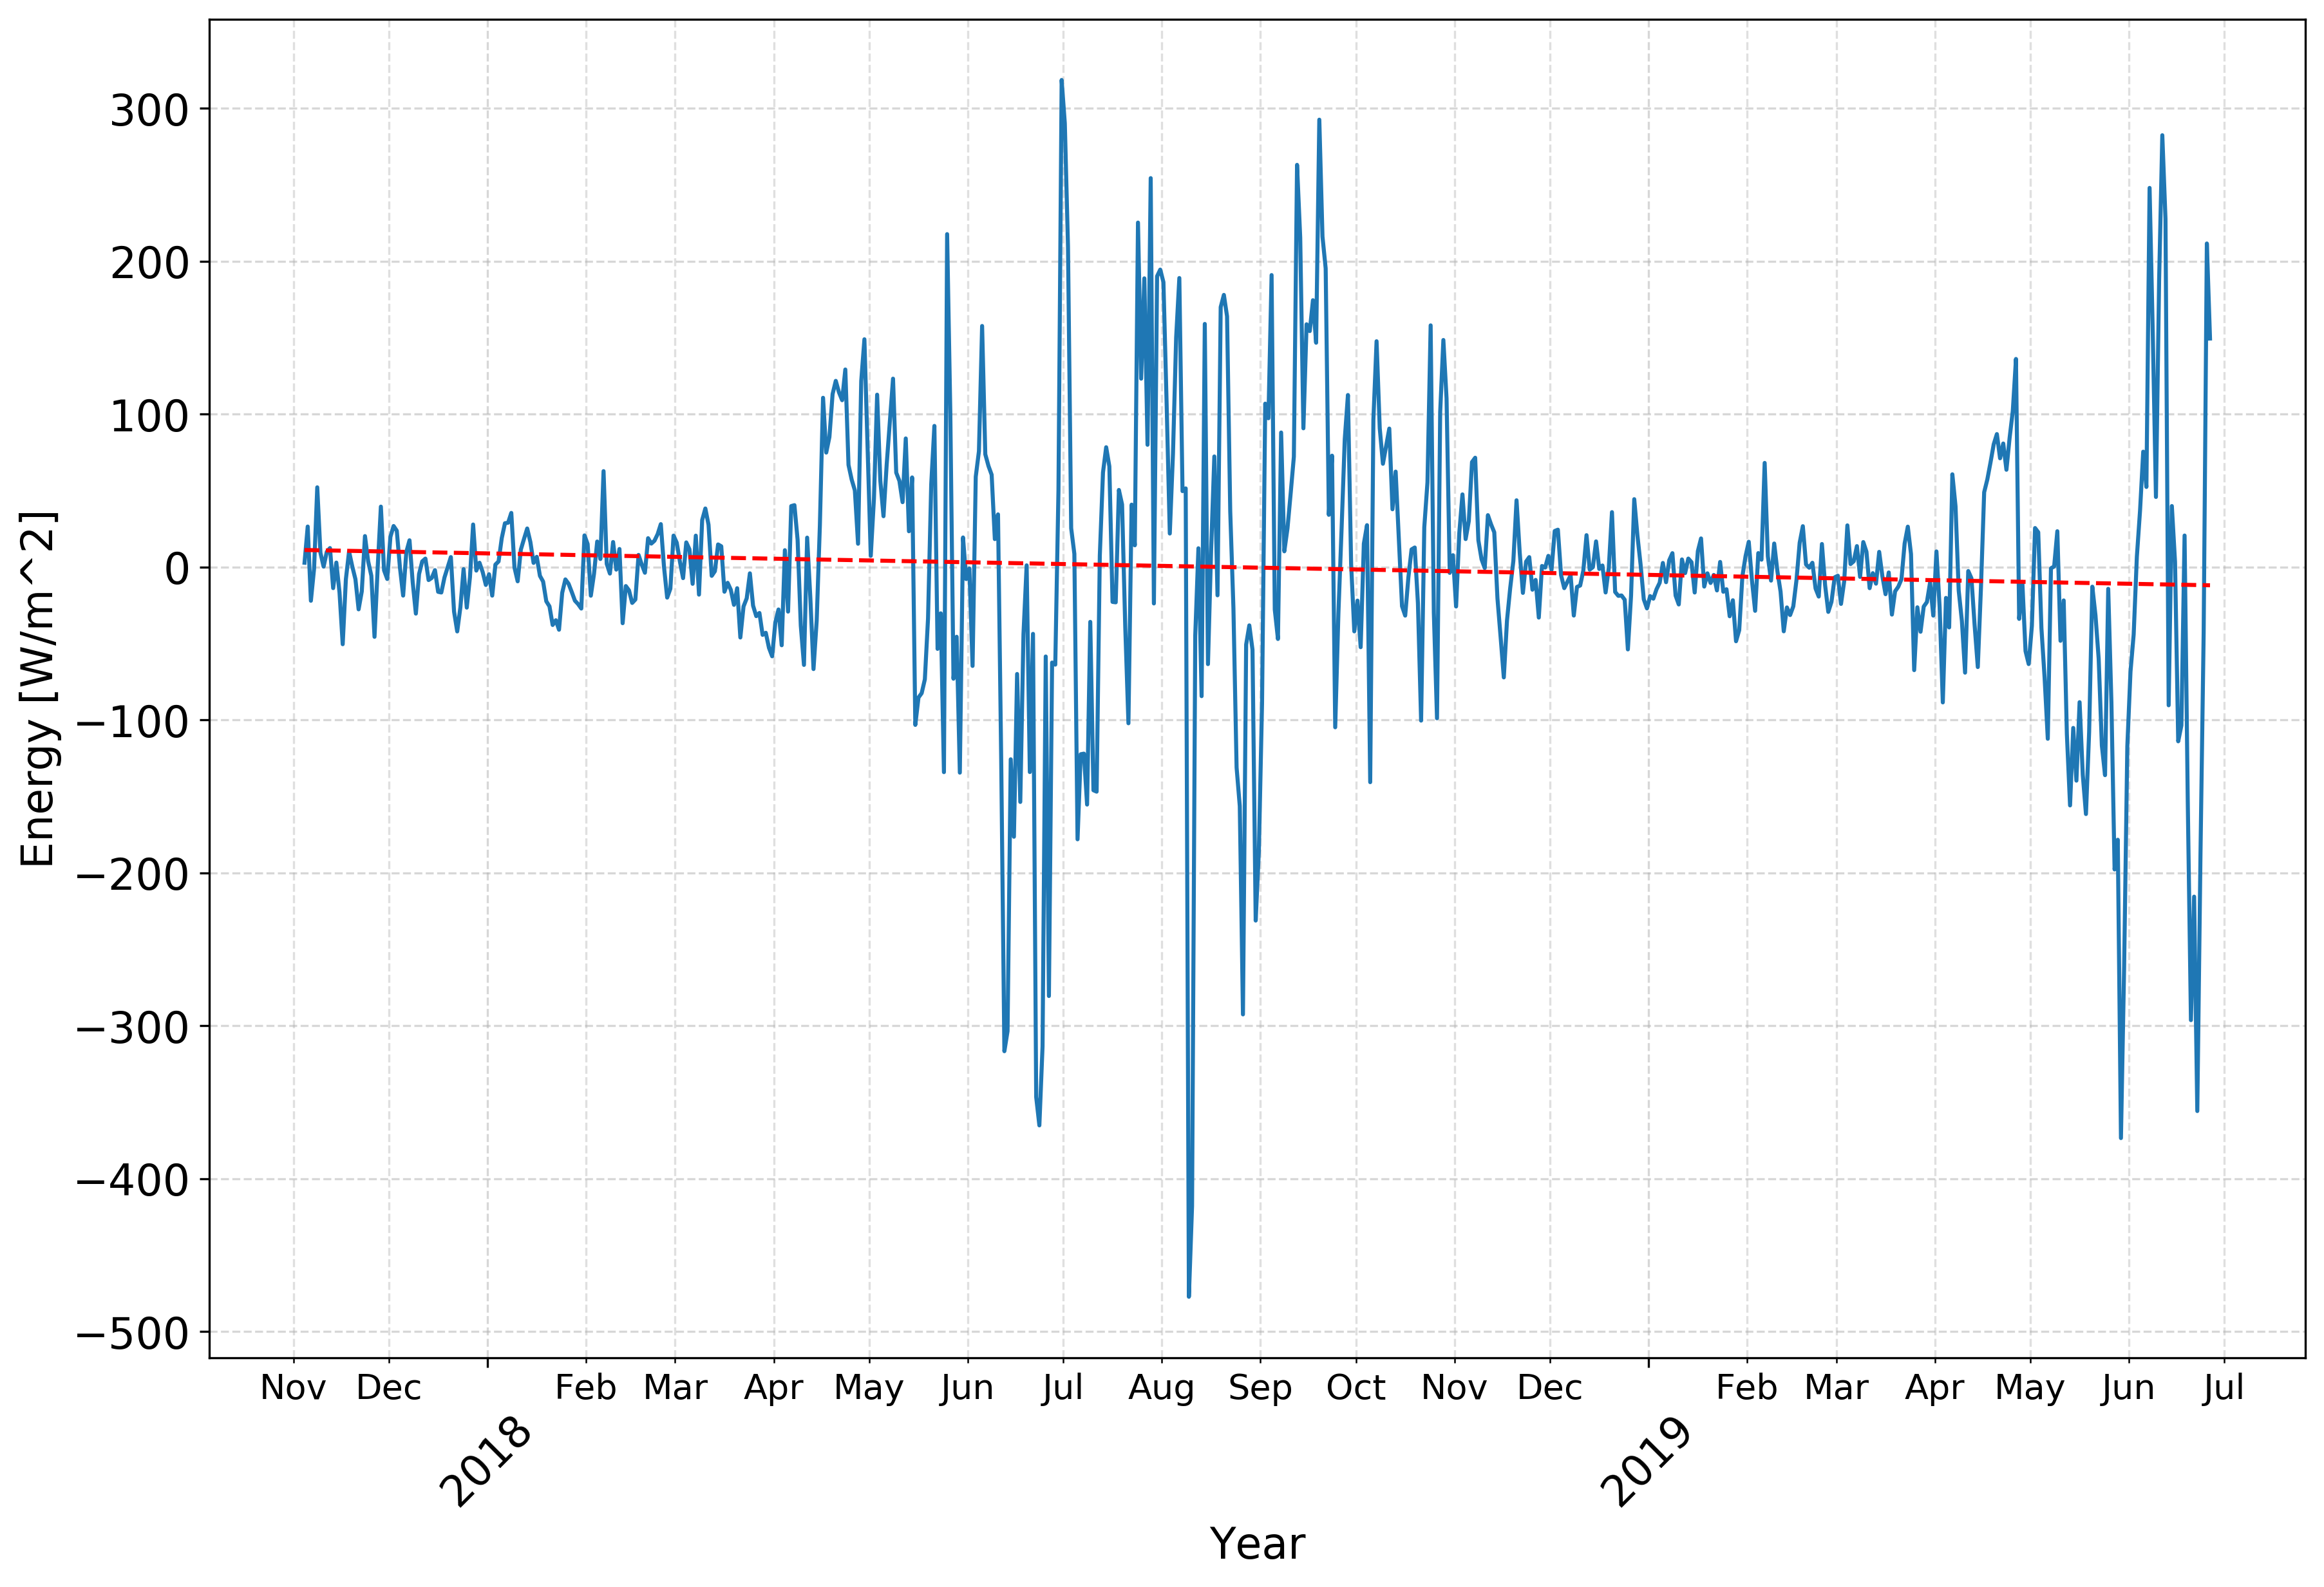
\includegraphics[width=1\textwidth]{../Software/plots/Total_energy_balance_summed_periodic_trend_eliminated.png}
\caption{Kompletter Zeitraum aufsummiert nur sensible und latent heat}
\label{fig:..}
\end{figure}

\begin{figure}[H]
\centering
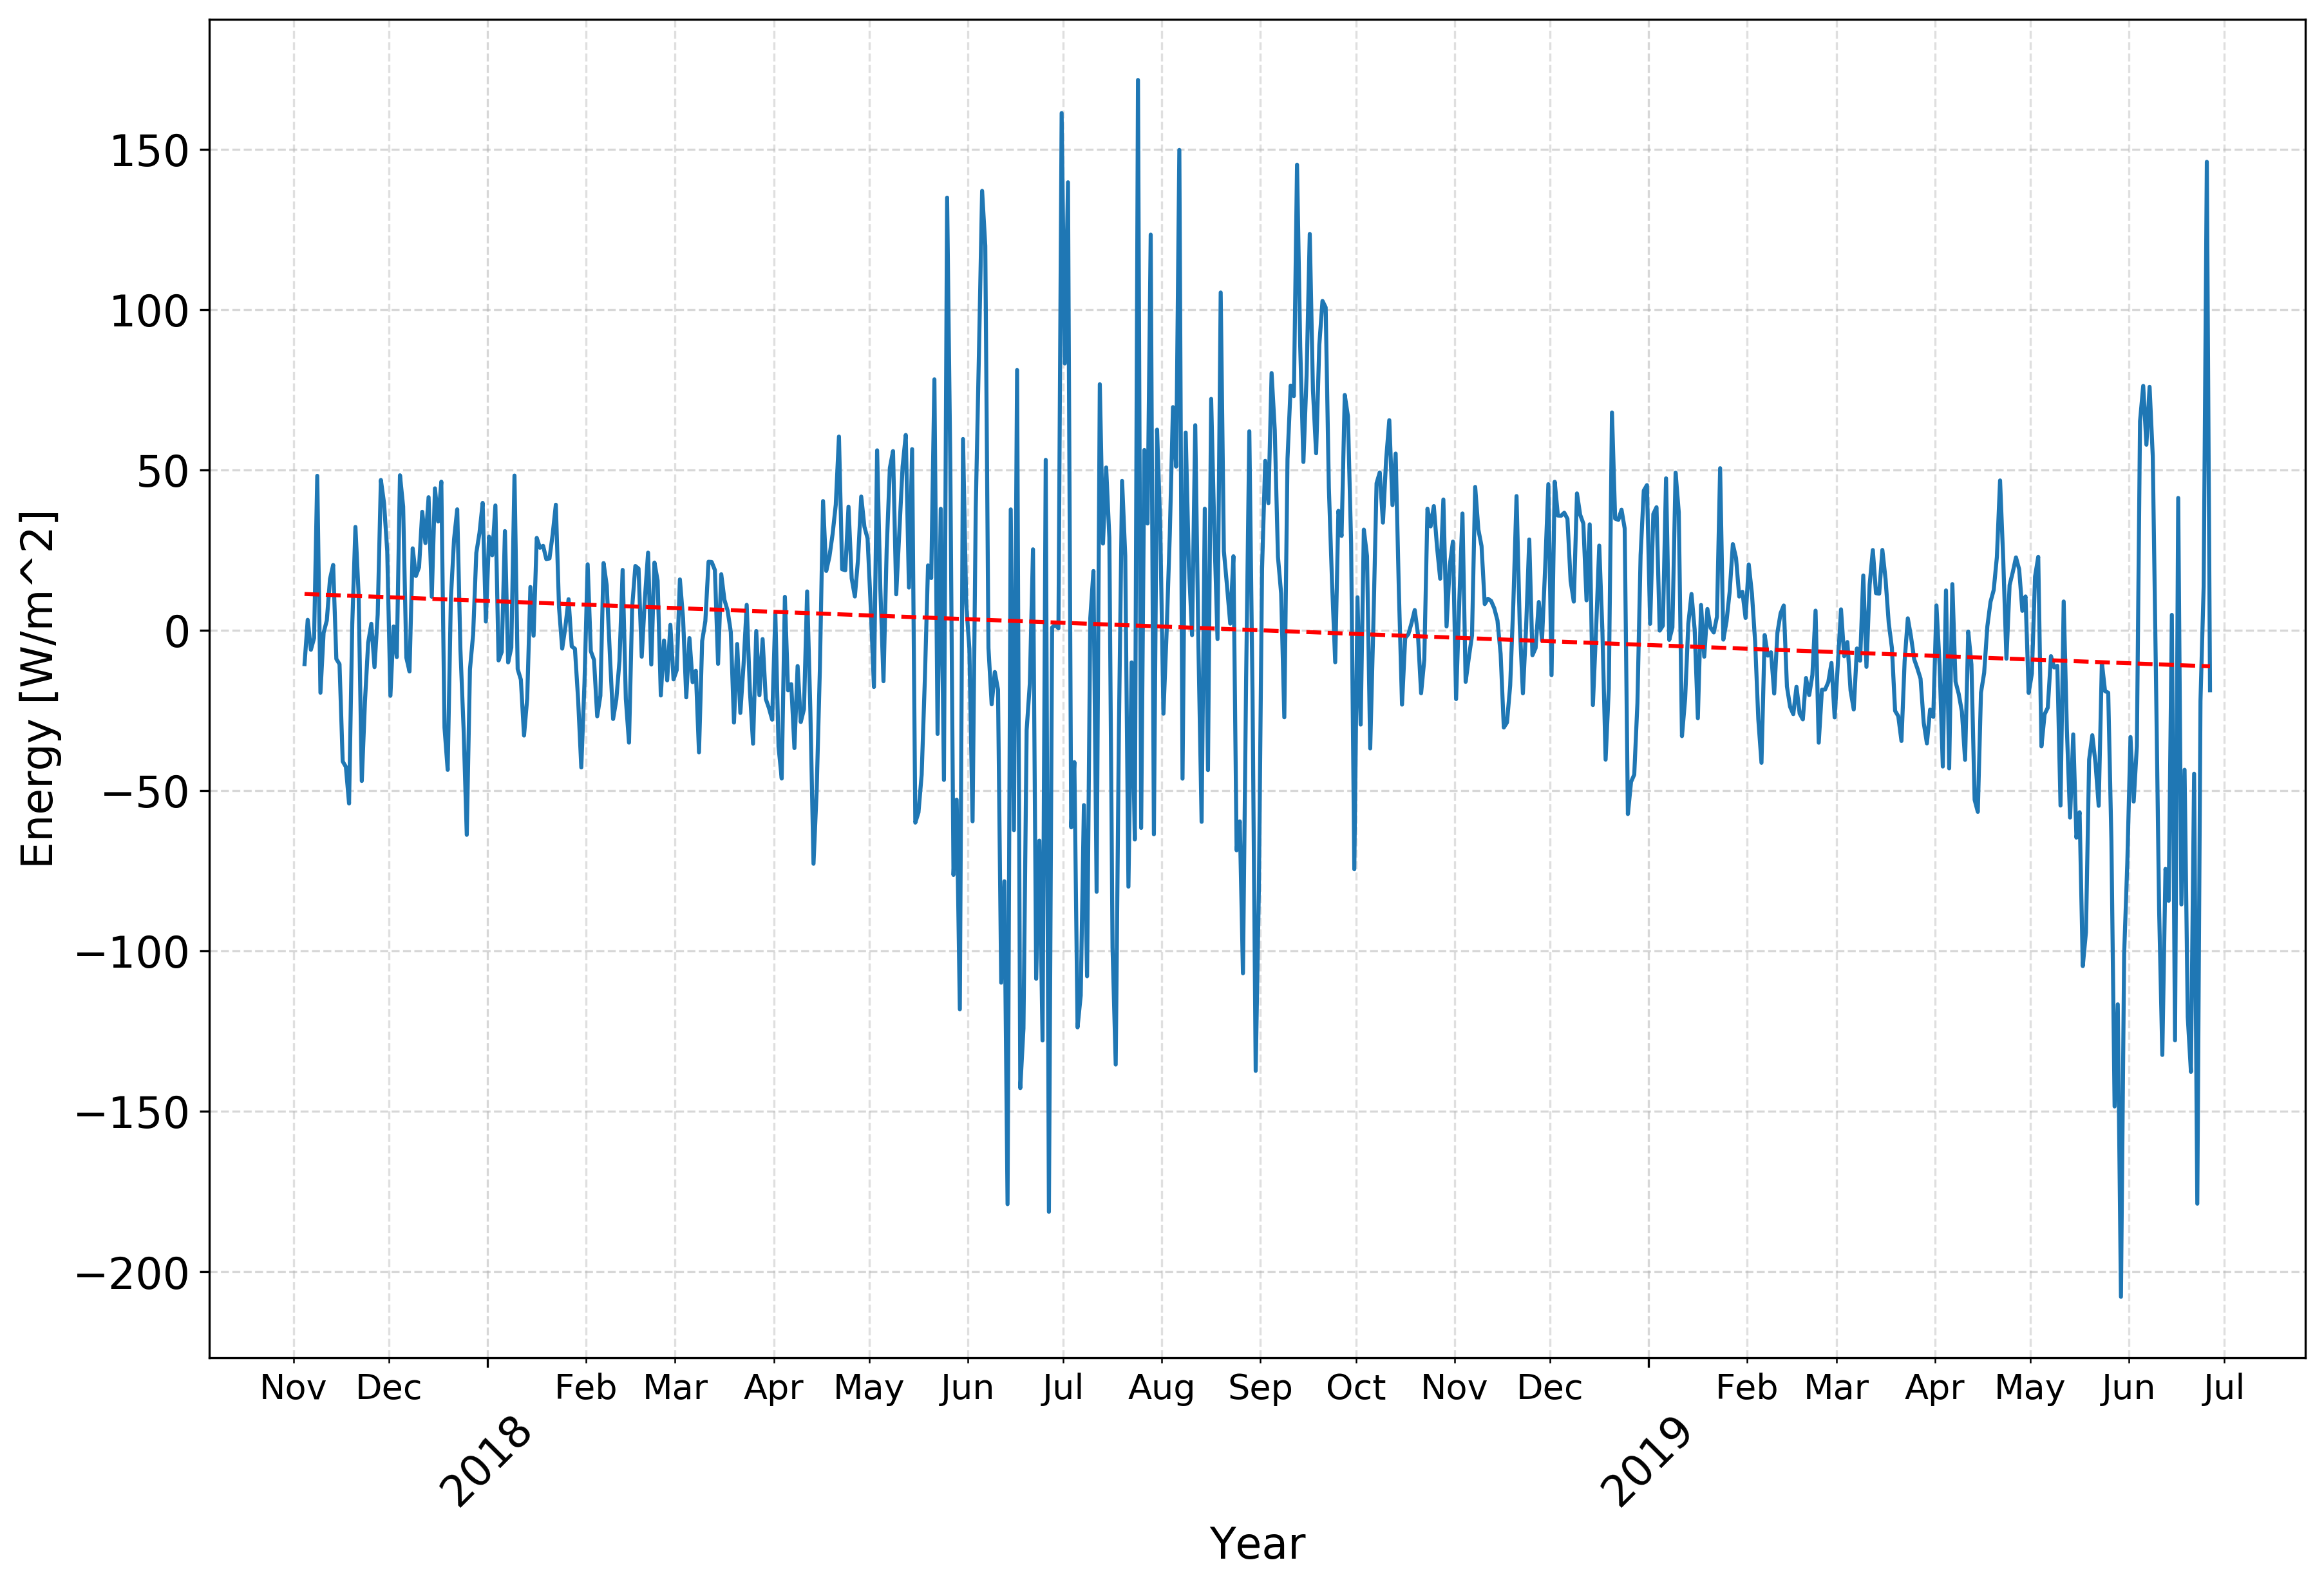
\includegraphics[width=1\textwidth]{../Software/plots/Radiation_summed_periodic_trend_eliminated.png}
\caption{Kompletter Zeitraum aufsummiert nur sensible und latent heat}
\label{fig:..}
\end{figure}

\begin{figure}[H]
\centering
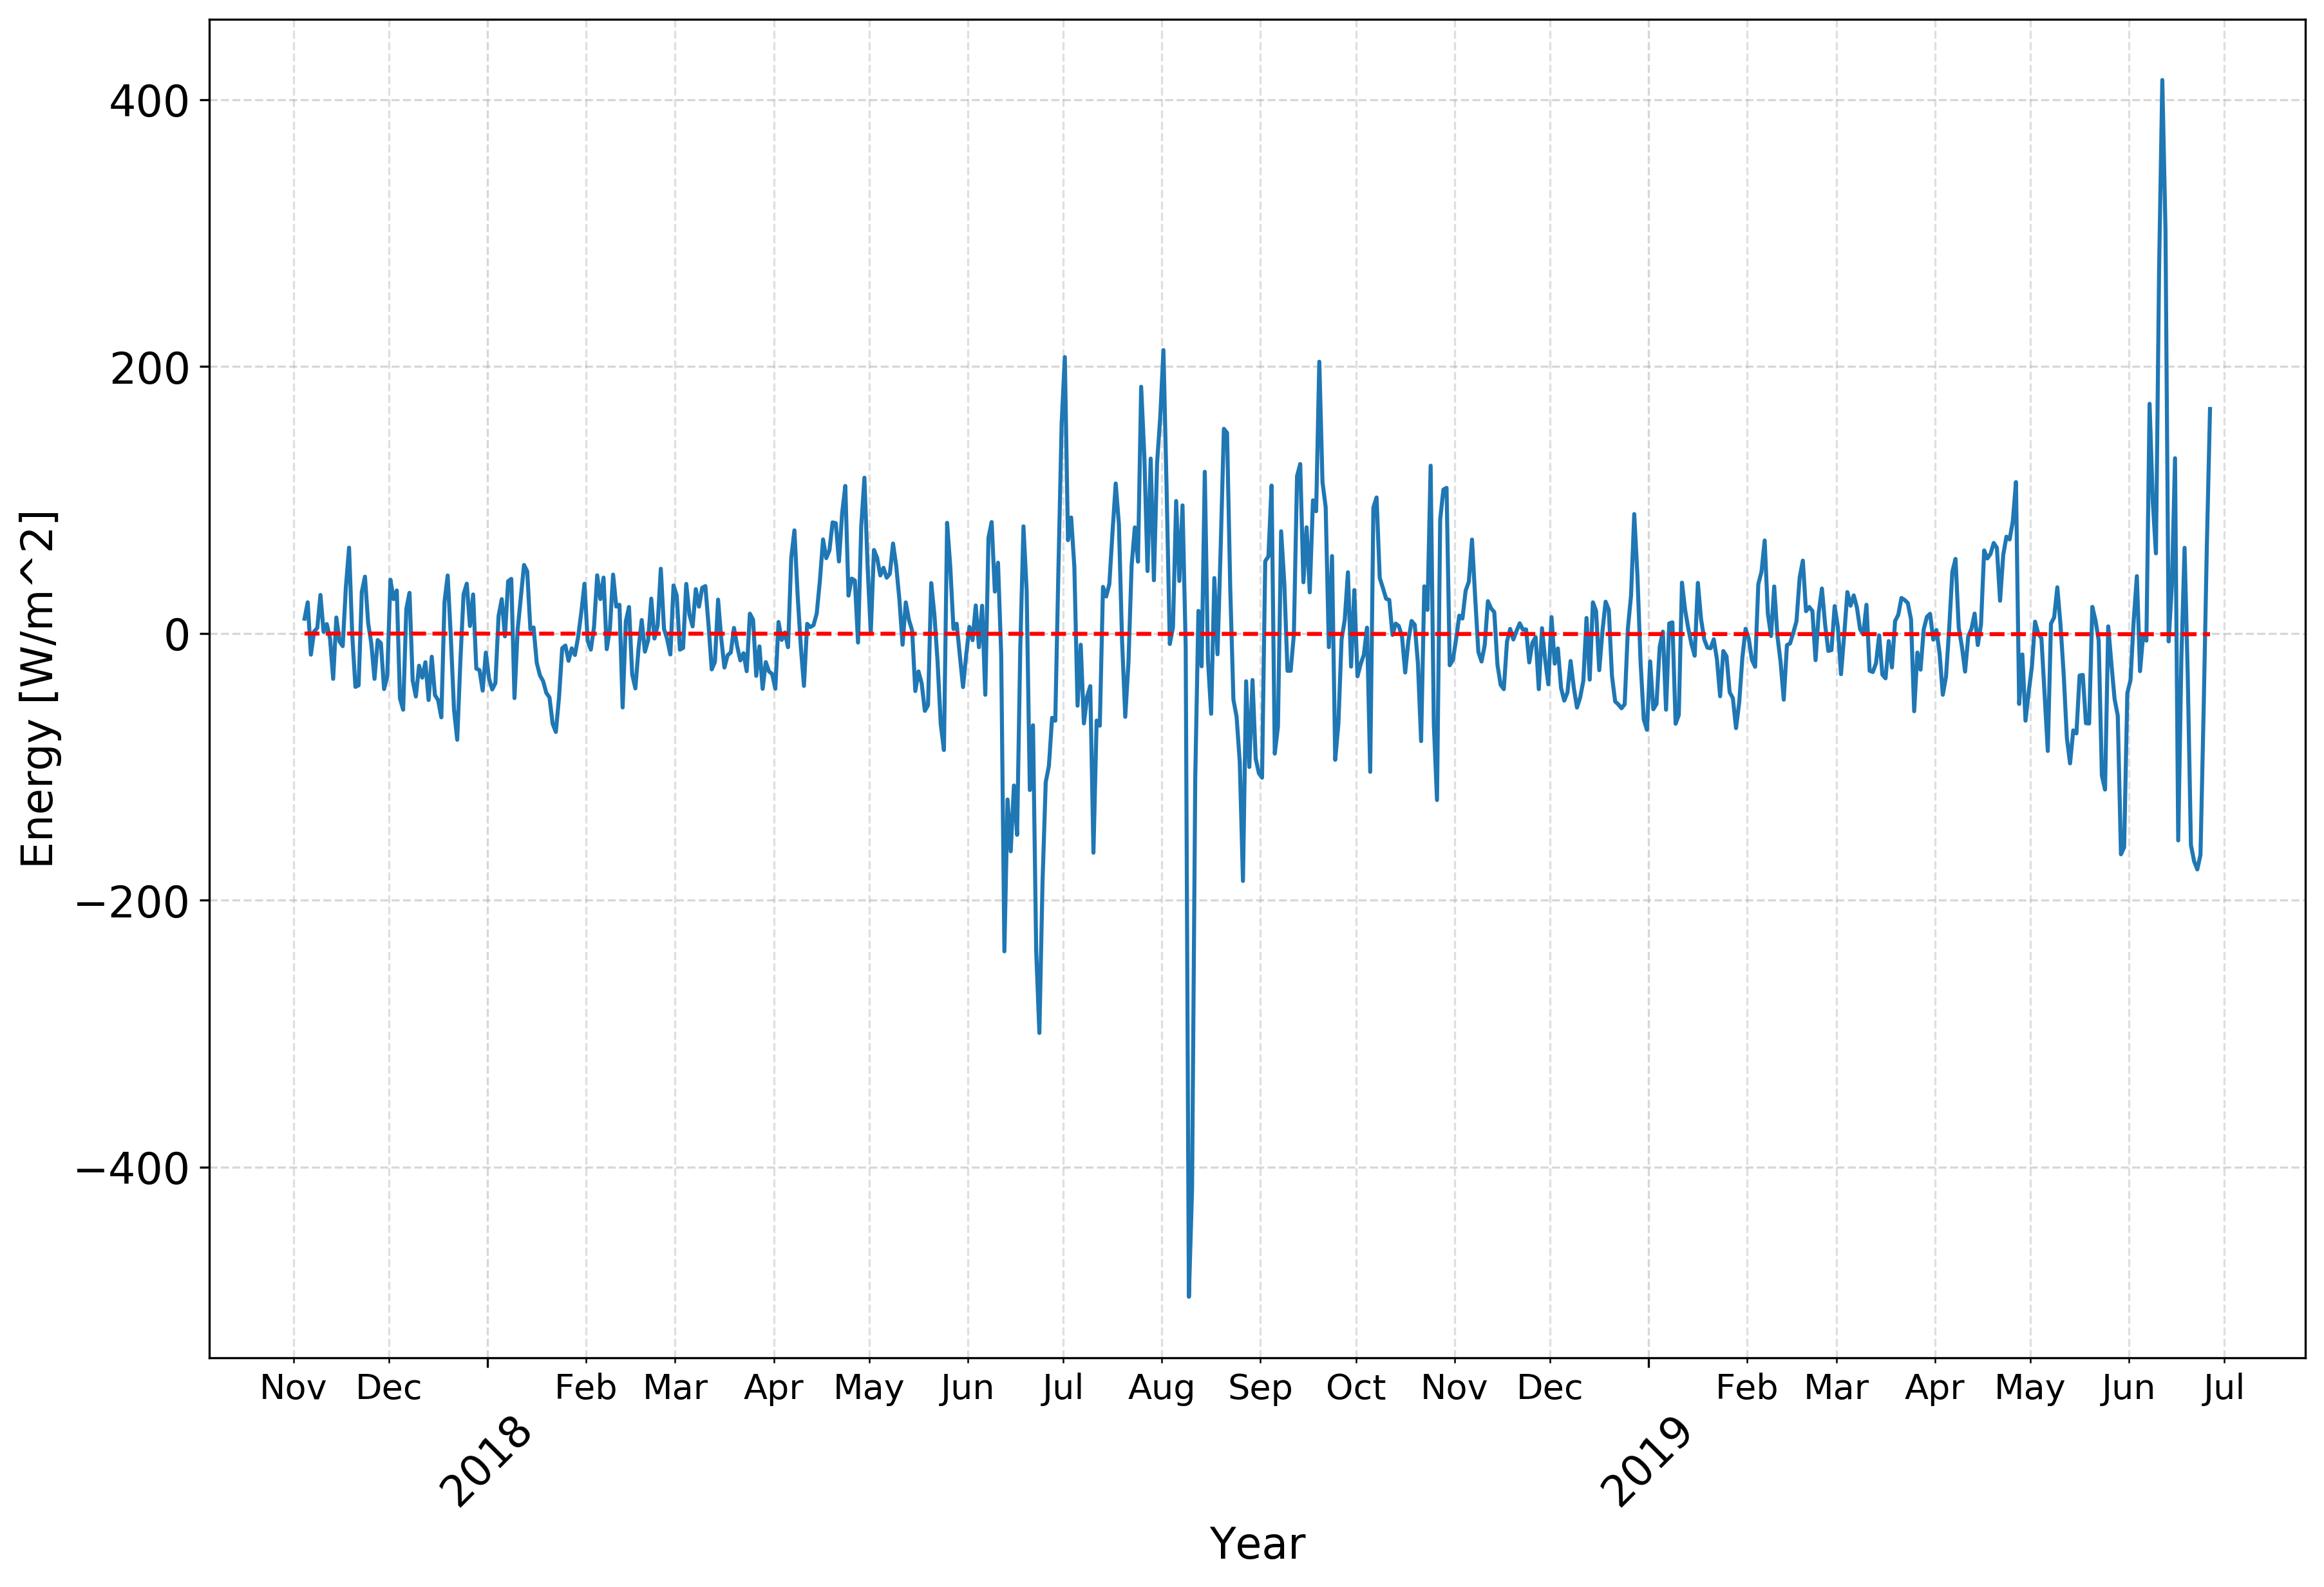
\includegraphics[width=1\textwidth]{../Software/plots/Latent_and_Sensible_summed_periodic_trend_eliminated.png}
\caption{Kompletter Zeitraum aufsummiert nur sensible und latent heat}
\label{fig:..}
\end{figure}



simulieren von global dimming brightening und schauen wie es sich im modelled meltwater auswirkt
modelled immer etwas mehr als beim wirklichen .. vor allem bei niedriger EB, welchen Grund könnte das haben?

beim simulieren von Global Dimming bzw. Global brightening wird das theoretische Schmelzwasser berechnet und in Eisäquivalent umgerechnet. Damit wird ein greifbarer Wert geliefert, wie viel das Eis bei diesem Phänomen tatsächlich an Eisdicke gewinnt bzw. verliert.




\pagebreak
\section{Fazit}


\section{Literaturverzeichnis}
%SELF MADE BIBLIOGRAPHIE IN GEOGRAPHIE GRAZ CITAVI STYLE
Cuffey, K.; Paterson, W. S. B. (2010): The physics of glaciers. 4th ed. Burlington MA: Butterworth-Heinemann/Elsevier.\\

Lieb, G. Karl; Slupetzky, H. (2011): Die Pasterze. Salzburg: A. Pustet.\\

Wakonigg, B.; Wakonigg, H.; Lieb, G. K.: Längenänderung der Pasterze. Hg. v. Institut für Geographie und Raumforschung. Online verfügbar unter https://geographie.uni-graz.at/de/forschung/forschungsgruppen/aladyn/projekte/pasterze/messergebnisse/laengenaenderung/, zuletzt geprüft am 10.06.2019.\\

Wild, M. (2009): Global dimming and brightening: A review. In: J. Geophys. Res. 114, 21, S. 1319. DOI: 10.1029/2008jd011470.



\end{document}